\documentclass[preprint]{elsarticle}
\usepackage{amssymb}
\setcounter{tocdepth}{3}
\usepackage{graphicx,epsfig}
\usepackage{graphicx}
\usepackage{algorithm}
\usepackage{algorithmic}
%\usepackage{listings}
\usepackage{rotating}
\usepackage{subfigure}
\usepackage{multirow}
%\usepackage[boxed]{algorithm2e}l
%\usepackage{algpseudocode}

\providecommand{\SetAlgoLined}{\SetLine}
\providecommand{\DontPrintSemicolon}{\dontprintsemicolon}
%%%%

\usepackage{color}
\usepackage{alltt}
\usepackage{verbatim}
\usepackage{moreverb} 
\usepackage{url}
%\usepackage[utf8]{inputenc}
\usepackage{inputenc}
%\usepackage[spanish]{babel}
\usepackage{url}

\begin{document}

\begin{frontmatter}

%%%%%%%%%%%%%%%%%%%%%%%%%%%%%%%   TITLE   %%%%%%%%%%%%%%%%%%%%%%%%%%%%%%%

\title{Analyzing the Influence of the Fitness Function on Genetically Programmed Bots for a Real-Time Strategy Game}
% What problem are we solving? Why do we need to test and analyse? - JJ
% Antonio - Mejorado
% What about genetically programmed bots? Or bots evolved via Genetic
% Programming? - JJ
% Antonio - Paso a hablar en cristiano que todos somos de Madrid pabajo. ;D
% Me ha gustado lo de 'Genetically-Programmed', a ver qu� opina Antares.

%%%%%%%%%%%%%%%%%%%%%%%%%%%%%%%   AUTHORS   %%%%%%%%%%%%%%%%%%%%%%%%%%%%%%%

\author{A. Fern{\'a}ndez-Ares, A.M. Mora, P. Garc{\'i}a-S{\'a}nchez, P.A. Castillo, J.J. Merelo}
\ead{\{antares, amorag, pgarcia, pedro, jmerelo\}@geneura.ugr.es}
%\address{Departamento de Arquitectura y Tecnología de Computadores.\\ ETSIIT - CITIC. University of Granada, Spain}
\address{Department of Computer Architecture and Technology\\ ETSIIT, CITIC. University of Granada, Spain}

%\maketitle

%
%%%%%%%%%%%%%%%%%%%%%%%%%%%%%%%%%   ABSTRACT   %%%%%%%%%%%%%%%%%%%%%%%%%%%%%%%%%
%
\begin{abstract}
% una o dos frases dando una breve introduccion general al area
Real-Time Strategy games (RTSs) are one of the common testbeds for research in the Computational Intelligence field.
% dos o tres frases mas detallando el background
The automatic generation of autonomous agents (bots) to play this kind of games is also a very prolific research line. However, the applied techniques to do this, must deal with uncertainty and real-time planning in order to control the game agents.
% una frase muy directa indicando el problema general a resolver en este trabajo
This work presents a Genetic Programming (GP) algorithm to create the behavioural engine of bots able to play an RTS. Three different fitness functions are proposed and a detailed analysis of their performance has been conducted. The aim is to get a better deal with this uncertainty. 
% una frase muy directa indicando el resultado obtenido en este trabajo (el mas destacable)
The results show that GP is a suitable method to generate bots to play a `simple' RTS game, Planet Wars. Moreover, it provides a mechanism to generate rules that enable to define very different behaviours.
% un par de frases indicando lo que aporta este resultado al estado del arte
The paper analyses several aspects of the bots, in addition to their final performance on battles, such as the evolution of the decision trees themselves, or the influence on the results of noise/uncertainty always present in the context of games.
% una ultima frase poniendo el resultado en un ambito general
As a general conclusion a victory-based fitness, which prioritises the number of victories, contributes to generate better bots, on average, than other functions based on the numerical aspects of the battles, such as the number of resources gathered, or the number of units generated. 
\end{abstract}
% Antonio - he hecho una mejora de lo que propon�a Pedro, atendiendo tambi�n a lo que suger�a JJ. A ver si os gusta. ;)
%
%%%%%%%%%%%%%%%%%%%%%%%%%%%%%%%%%   KEYWORDS   %%%%%%%%%%%%%%%%%%%%%%%%%%%%%%%%%
%
\begin{keyword}
Real-time Strategy game \sep Genetic Programming \sep Autonomous agent \sep Bot \sep Fitness function \sep Uncertainty
\end{keyword}

\end{frontmatter}


%-------------------------------------------------------------------
%%%%%%%%%%%%%%%%%%%%%%%% INTRODUCTION %%%%%%%%%%%%%%%%%%%%%%%%%%%%%%
%-------------------------------------------------------------------
\section{Introduction}
\noindent 

Real-Time Strategy (RTS) games are a genre of videogames where the action takes place in a scenario (or arena) and the contenders must fight, controlling a set of units, in order to monopolise the resources and, eventually, to defeat the opponent. These games are not turn-based, so the players must take decisions in real-time. This kind of games has become an interesting testbed in Computational Intelligence research \cite{Lara2013review}, as they can be seen as a simplification of more complex scenarios, such as road traffic simulation or financial prediction. As in these environments, in addition to the required real-time planning, there is some uncertainty present in RTSs.

In this scope, the automatic generation of agents (also called {\em bots}) to play this kind of games is one of the most prominent areas. For example, Evolutionary Algorithms (EAs) have been previously used for the creation of bots/strategies in RTSs such as {\em Planet Wars} \cite{Genebot_CEC11,ExpGenebot_CIG2012,Garcia14Treedepth} or {\em StarCraft} \cite{bistrom_GP_StarCraft,Barriga2014:BuildingOrder_GA,Garcia15Starcraft}, among others. 

% Antonio - introduzco aqu� lo que son los EAs, porque viene bien para justificar la importancia del fitness. ;D
EAs \cite{EAs_Back96} are a class of probabilistic search and optimisation algorithms inspired on the model of Darwinistic evolution. 
There are several subtypes, depending on the data structure that is preferentially used for representing solutions, but Genetic Algorithms (GAs) \cite{GAs_Goldberg89} and Genetic Programming (GP) \cite{GP_Koza92} are the most extended. The main features are common to all of them: a population of individuals or potential solutions of the target problem, a selection method that favours better solutions, and a set of operators that act upon the
selected solutions. Thus, after an initial population is created (usually random), the selection and operators - crossover and mutation - are applied to the individuals, and the new population then replaces the older one. This is repeated for a number of generations or until another stop condition is met. 
If there is defined a correct {\em fitness function}, which assigns a reliable value to every individual, this process guarantees that the average quality of the population increases with the number of generations.
Thus, deciding the best evaluation function is a key factor for the success of these algorithms.

The aforementioned works apply GAs \cite{Genebot_CEC11,ExpGenebot_CIG2012,Barriga2014:BuildingOrder_GA}, and GP \cite{bistrom_GP_StarCraft,Garcia14Treedepth,Garcia15Starcraft}. 
All these approaches have in common the consideration of an evaluation function which measures the quality of the behaviour of the bots being evolved. 
Different fitness functions have been used in the past, for example the {\em game score}, or the {\em number of victories} against the rivals during the evaluation. However, these functions have to deal with the uncertainty, also called {\em noise} \cite{merelo14:noisy,merelo15:uncertainty}, present due to the stochastic nature of the bots or to the game itself. 

In addition, the selection of a fitness function or another, may generate different behaviours for the generated bots. For example, an evolutionary process using a victory-based fitness function would create `aggressive' bots, while one function, that also takes into account the number of different structures created, may generate a more `strategic' bot. 

Therefore, this paper aims to choose the best type of fitness function for a Genetic Programming-based approach, which generates {\em Decision Trees} - or rule-based systems - (DTs), as Artificial Intelligence engines for bots in the scope of RTSs.
To this end, we compare the bots created using different types of fitness, studying both, the generated DTs, and the performance of the bots in battles against unknown enemies. 
We have applied GP to generate the bots because it provides a good mechanism to create rules from scratch, giving the possibility to define very different behaviours. 

Three fitness functions have been tested in the paper:
\begin{itemize}
\item A {\em victory-based fitness}, that only considers the number of battles won in the evaluation. %ANTARES: También tiene en cuenta los turnos, pero para desempatar...
% Antonio - mejor decirlo cuando se describa en detalle, para no liar aqu�. ;)
\item A {\em slope-based fitness}: that measures the behaviour during all the game (not only at the end, as in the previous one), using the slope of the number of generated units during the game.
\item An {\em area-based fitness}: which computes an integral as the average number of generated units divided by the number of turns the battle has taken. 
%PABLO: por qu? esta diferenciaci?n en estas dos ultimas?
%ANTARES: Realmente se calcula el número promedio de recursos en el número de turnos, y esto se calcula con la integral (sumatoria de valores discretos) dividido por el número de turnos
% Antonio - mirad si lo he descrito bien. ;)
\end{itemize}

These approaches have been implemented for the game {\em Planet Wars} (or Galcon
\cite{wiki:galcon}), as it is a `simple' RTS: with only one type of resources and units. 

%The presented paper is an extension of the paper published in \cite{Ares14Cosecivi}. 
% Antonio - Yo esto no lo mencionar�a, si acaso en alg�n punto se puede hacer la referencia, pero sin decir que es una extensi�n, ya que esto acarrea m�s problemas que otra cosa. Al decir que es una extensi�n hay que aclarar bien en qu� se extiende y justificar la necesidad de esta extensi�n. Los revisores ya lo saben y si lo piden lo ponemos. ;D
The rest of the paper is structured as follows: after the background and the problem description (Section \ref{section:background}), the state of the art is presented in Section \ref{sec:soa}. Then, the description of the GP approach and the considered fitness functions are described respectively in Sections \ref{sec:agent} and \ref{sec:fitness_functions}. Section \ref{sec:experiments} explains the experimental setup, while Section \ref{sec:results} analyses the obtained results. Finally, the conclusions and future lines work are presented in Section \ref{sec:conclusion}.



%-----------------------------------------------------------------
%%%%%%%%%%%%%%%%%%%%%%%% BACKGROUND %%%%%%%%%%%%%%%%%%%%%%%%%%%%%%
%-----------------------------------------------------------------
\section{Background and problem description}
\label{section:background}
\subsection{Genetic Programming}

Genetic Programming (GP) \cite{GP_Koza92} is a type of EA where the individuals are represented as hierarchical structures (typically trees), which size and shape is not defined a priori, as in other evolutionary methods, but they evolve along the generations. Thus, GP performs a structural optimisation, which requires the use of specific genetic operators, focused on the management (and improvement) of this kind of structure.
The flow of a GP algorithm is the same as any other EA: a population is created at random, each individual in the population is evaluated using a fitness function, the individuals that performed better in the evaluation process have a higher probability of being selected as parents for the new population, and a new population is created by applying crossover and mutation operators with a certain probability. This process is repeated until a predefined termination criterion is met.

% ----------------------------------------------------------------------

\subsection{Planet Wars Game}
In this paper we work with a %simplified
version of the game Galcon, aimed at performing bot's fights which was used for the Google AI Challenge 2010 (GAIC)\footnote{http://planetwars.aichallenge.org/}.

 \begin{figure}[ht]
 \begin{center}
   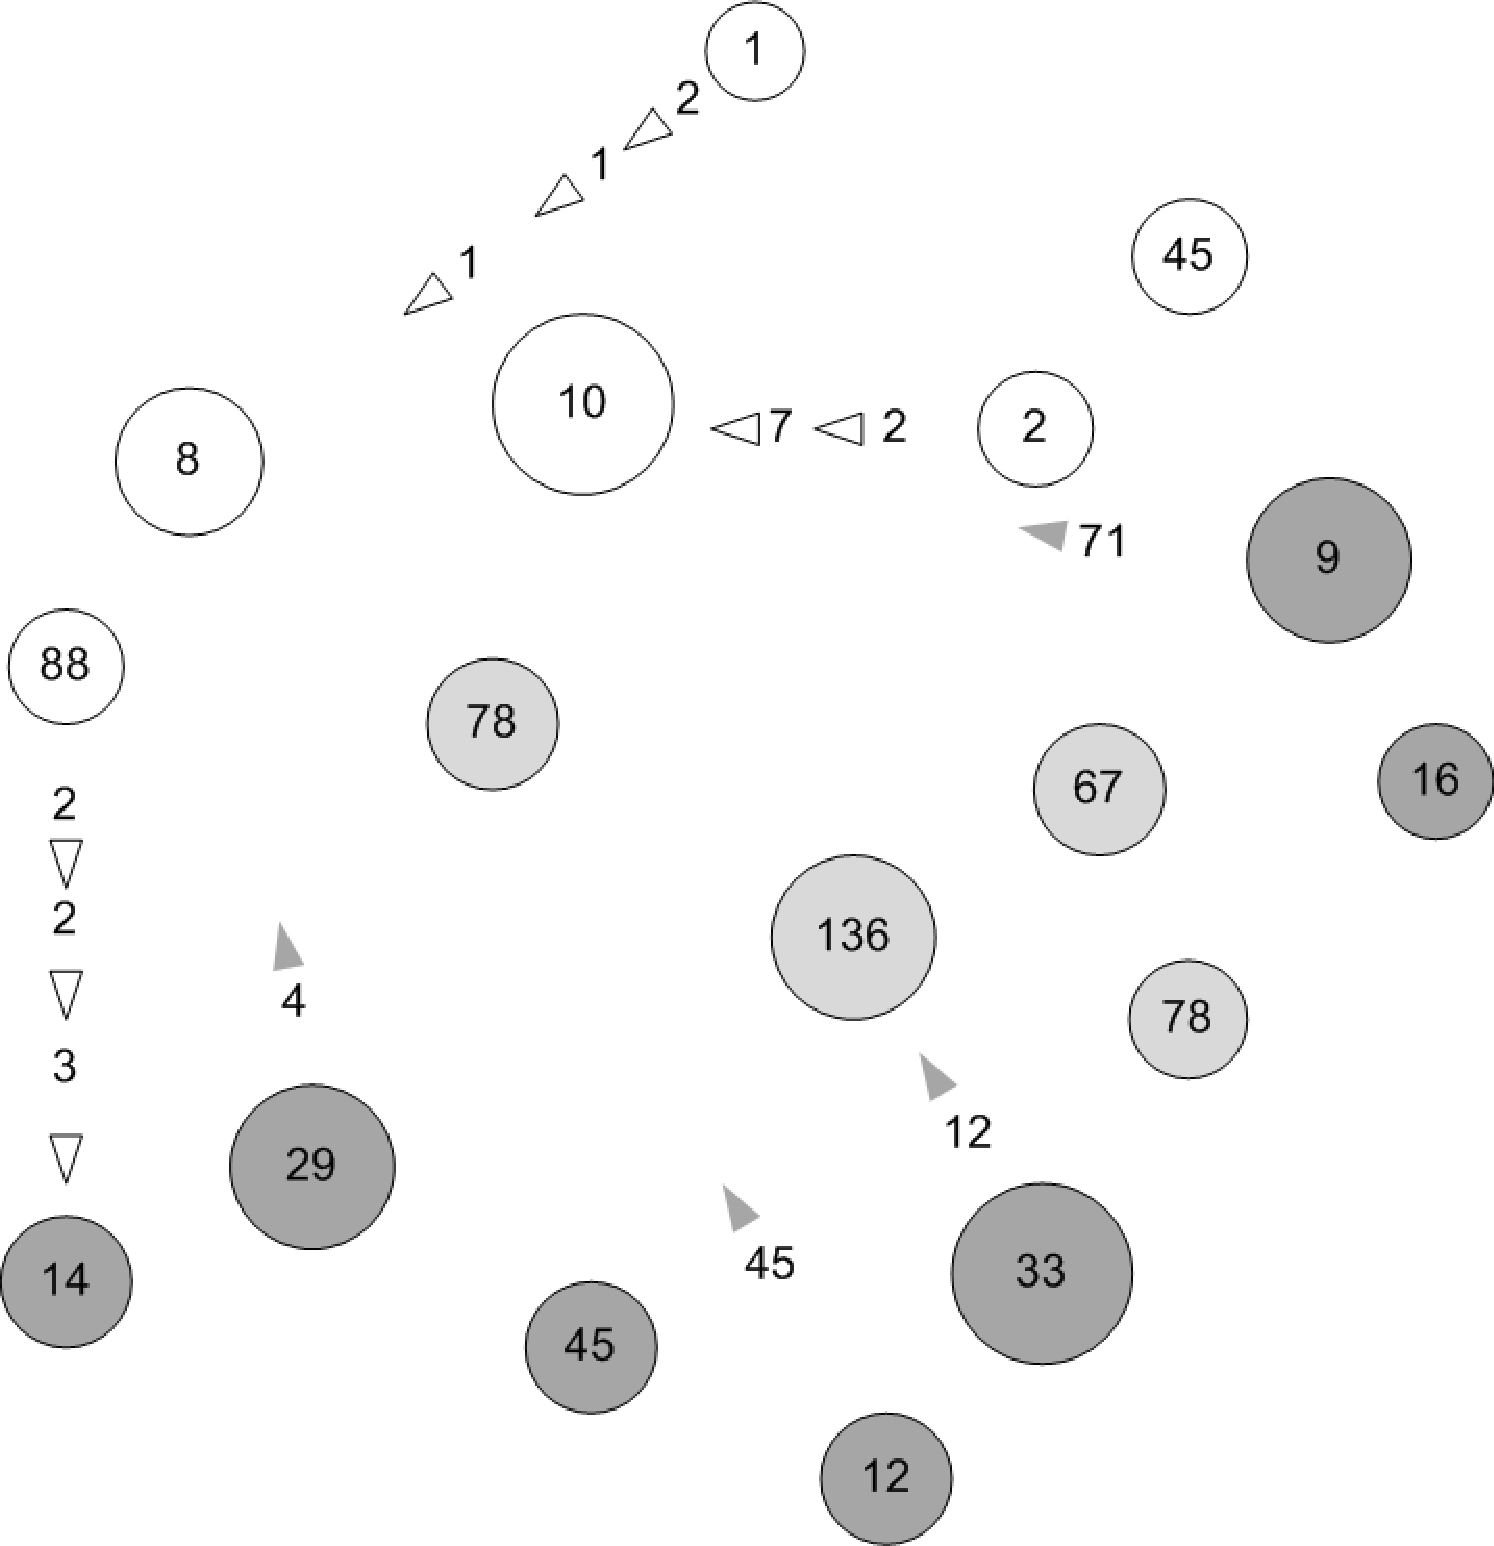
\epsfig{file=./imags/naves.pdf,width=7cm}
 \end{center}
 \caption{Simulated screenshot of an early stage of a run in Planet Wars. White planets belong to the player (blue colour in the game), dark grey belong to the opponent (red in the game), and light grey planets belong to no player. The triangles are fleets, and the numbers (in planets and triangles) represent the ships. The planet size means growth rate of the amount of ships in it (the bigger, the higher).}
 \label{figura:PlanetWars1}
 \end{figure}

A Planet Wars match takes place on a map (see Fig. \ref{figura:PlanetWars1})
that contains several planets (neutral, enemies, or owned), each one of them with a number assigned to it that represents the amount of ships that the planet is currently hosting. 

The aim of the game is to defeat all the ships in the opponent's planets. Although Planet Wars is a RTS game, this implementation has transformed it into a turn-based game, in which each player has a maximum number of turns to accomplish the objective. At the end of the match, the winner is the player that remains alive, or that which owns more ships if more than one survives. 

There are two strong constraints which determine the possible methods to apply to design a bot: the time for making a decision is \textit{just one second}, 
and the bot is \textit{not allowed to store any kind of information} about its former actions, about the opponent's actions or about the state of the game (i.e., the game's map). 

Therefore, the objective of this paper is to generate a reliable DT for a bot, which, according to the state of the map in every simulated turn (input), returns a set of actions to perform in order to fight the enemy, conquer its resources, and finally, win the game. 


%-----------------------------------------------------------------------
%%%%%%%%%%%%%%%%%%%%%%%% STATE OF THE ART %%%%%%%%%%%%%%%%%%%%%%%%%%%%%%
%-----------------------------------------------------------------------
\section{State of the art}
\label{sec:soa}

RTS games have been used extensively in the Computational Intelligence (CI) area (see \cite{Lara2013review} for a survey). 
Among other techniques, EAs have been widely used as a CI method in RTS games, for example, for parameter optimisation \cite{Genebot_CEC11,ExpGenebot_CIG2012}, building order decision \cite{Kostler2013:MO_StarCraftII,Barriga2014:BuildingOrder_GA}, learning \cite{learning_StarCraft_AAIDE11,Wender_RL_CIG12}, or content generation \cite{Mahlmann2012MapGeneration,Lara_EntComp_PCG_RTS14}. 

GP has also proved to be a very good tool for developing strategies in games, achieving results comparable to human, or human-based competitors \cite{Sipper2007gameplaying}. They also have obtained higher ranking than solvers produced by other techniques or even beating expert human players \cite{Elyasaf2012FreeCell}. GP has also been used in different kind of games, such as board-games \cite{Benbassat2012Reversi}, (apparently) `simple' games like Ms. Pac-Man \cite{Brandstetter2012PacMan} or Spoof \cite{Wittkamp2007spoof}, and even in modern videogames such as First Person Shooters (FPS) as Unreal\texttrademark~ \cite{Mora_UnrealBots10,Esparcia2013GPunreal}. 

With respect to RTS games, it has not been extremely exploited, so there are just a few applications, such as pathfinding \cite{pathfinding_GP_RTS}, definition of tactics in an abstract tactical game \cite{KeaveneyO09_GP_RTS},and recently to the automatic generation of strategies for a bot \cite{Garcia15Starcraft}.
% Antonio - Fergu, mira a ver si quieres a�adir algo a esto. ;)
In this paper, the aim is to apply GP inside a `simple' RTS, Planet Wars, in order to define the whole behavioural engine for bot.
 
Planet Wars, the game used in this work, has also been used in other researches as an experimental framework for agent testing. 
We have considered this game in some previous studies \cite{Genebot-IWANN2011,Genebot_CEC11,genebot-evo12,ExpGenebot_CIG2012,Co-Genebot_EVO2014}, mainly applying Genetic Algorithms for evolving (the parameters of) a behavioural engine previously defined by a human expert from scratch. Those works have respectively defined a first approach, compared different implementations, analysed the noise influence, defined expert bots, and implemented co-evolutionary approaches.

% TODO: *** METER COSAS DE EN QU� AVANZA ESTE ART�CULO EL SotA: 
% - Estudio en profundidad de los �rboles (que antes no se hab�a hecho)
% - �Mejora en los resultados?
% - �Algo del ruido?

%For example, in
%\cite{Mora2012Genebot} the authors programmed the behaviour of a {\em bot} (a computer-controlled player) with a decision tree of 3 levels. Then, the values of these rules were optimized using a genetic algorithm to tune the strategy rates and percentages.  
%  Results showed a good performance confronting with other bots
%  provided by the Google AI Challenge. %In our next work
%  In \cite{FernandezAres2012adaptive} the authors improved this agent optimizing it in different types of maps and selecting the set of optimized
%  parameters depending on the map where the game was taking place,
%  using a tree of 5 levels. These results outperformed the previous
%  version of the bot with 87\% of victories. 

The present work means a new step in this research line, which tries to avoid the strict limitations that the initial bot had, i.e. since it was defined by a human expert, it had a fixed structure (a Finite State Machine) which just offers a few degrees of improvement, namely a set of eight parameters.
The use of GP here will provide us with a new tool for completely redefine the bot's AI engine, which could also get better results than previous bots.
Thus GP has been applied to create the Decision Tree that the bot will use to make decisions during the game.
In order to prove the method value, the resulting agents will be compared with a competitive bot previously presented: GeneBot \cite{Genebot_CEC11}, our initial bot improved by means of Genetic Algorithms. This bot also proved (in that work) to be better than a human-defined bot (AresBot).
% AntonioDEF - He completado esto un poco para justificar mejor el trabajo. Comento además que Genebot era mejor que uno definido por un humano, Aresbot.



%-------------------------------------------------------------
%%%%%%%%%%%%%%%%%%%%%%%% GP BOT %%%%%%%%%%%%%%%%%%%%%%%%%%%%%%
%-------------------------------------------------------------
\section{GPBot}
\label{sec:agent}


The Genetic Programming-based bot or {\em GPBot} \cite{Garcia14Treedepth} evolves a set of rules which, in turn, models a Decision Tree (DT).

During the evolution, every individual in the population (a tree) must be evaluated. To do so, the tree is set as the behavioural engine of an agent, which is then placed in a map against a rival in a Planet Wars match. Depending on the obtained results, the agent (i.e. the individual) gets a fitness value, that will be considered in the evolutionary process as a measure of its validity. 
 
Thus, during the match the tree will be used (by the bot) in order to select the best strategy at every moment, i.e. for every planet a target will be selected along with the number of ships to send from one the other.

\noindent The used DTs are binary trees of expressions composed by two different \textit{types of nodes}:

\begin{itemize}
\item {\em Decision}: a logical expression formed by a variable, a less than operator ($<$), and a number between 0 and 1. It is the equivalent to a ``primitive'' in the field of GP.
\item {\em Action}: a leave of the tree (therefore, a ``terminal''). Each decision is the name of the method to call from the planet that executes the tree. This method indicates to which planet send a percentage of available ships (from 0 to 1). 
\end{itemize}

\noindent The decisions are based in the values of different \textit{variables} which are computed considering some other variables in the game. They are defined by a human expert, and are:

\begin{itemize}
\item {\em myShipsEnemyRatio}: Ratio between the player's ships and enemy's ships.
\item {\em myShipsLandedFlyingRatio}: Ratio between the player's landed and flying ships.
\item {\em myPlanetsEnemyRatio}: Ratio between the number of player's planets and the enemy's ones.
\item {\em myPlanetsTotalRatio}: Ratio between the number of player's planet and total planets (neutrals and enemy included).
\item {\em actualMyShipsRatio}: Ratio between the number of ships in the specific planet that evaluates the tree and player's total ships.
\item {\em actualLandedFlyingRatio}: Ratio between the number of ships landed and flying from the specific planet that evaluates the tree and player's total ships.
\end{itemize}

\noindent Finally, the possible \textit{decisions} are:

\begin{itemize}
\item {\em Attack Nearest (Neutral|Enemy|NotMy) Planet}: The objective is the nearest planet.
\item {\em Attack Weakest (Neutral|Enemy|NotMy) Planet}: The objective is the planet with less ships.
\item {\em Attack Wealthiest (Neutral|Enemy|NotMy) Planet}: The objective is the planet with higher lower rate.
\item {\em Attack Beneficial (Neutral|Enemy|NotMy) Planet}: The objective is the  more beneficial planet, that is, the one with highest growth rate divided by the number of ships.
\item {\em Attack Quickest (Neutral|Enemy|NotMy) Planet}: The objective is the planet easier to be conquered: the lowest product between the distance from the planet that executes the tree and the number of  ships in the objective planet.
\item {\em Attack (Neutral|Enemy|NotMy) Base}: The objective is the planet with more ships (that is, the base).
\item {\em  Attack Random Planet}.
\item {\em Reinforce Nearest Planet}: Reinforce the nearest player's planet to the planet that executes the tree.
\item {\em Reinforce Base}: Reinforce the player's planet with higher number of ships.
\item {\em Reinforce Wealthiest Planet}: Reinforce the player's planet with higher grown rate.
\item {\em Do nothing}.

\end{itemize}

\noindent An example of a possible DT is shown below. This example tree has a total of 5 nodes, with 2 decisions and 3 actions, and a depth of 3 levels.

\begin{verbatim}

if(myShipsLandedFlyingRatio < 0.796)
   if(actualMyShipsRatio < 0.201)
      attackWeakestNeutralPlanet(0.481);
   else
      attackNearestEnemyPlanet(0.913);
else
   attackNearestEnemyPlanet(0.819);

\end{verbatim}\\\\

\noindent The bot's behaviour is explained in Algorithm \ref{alg:turn}.

\begin{algorithm}[ht]
\begin{algorithmic}
%\SetAlgoLined
%\KwData{this text}
%\KwResult{how to write algorithm with \LaTeX2e }

\STATE // At the beginning of the execution the agent receives the tree
\STATE tree $\leftarrow$ readTree()
\WHILE{game not finished}
	\STATE // starts the turn
	\STATE calculateGlobalPlanets() // e.g. Base or Enemy Base
	\STATE calculateGlobalRatios() // e.g. myPlanetsEnemyRatio
	\FOR{Each p in PlayerPlanets}
		\STATE calculateLocalPlanets(p) // e.g. NearestNeutralPlanet to p
		\STATE calculateLocalRatios(p) //e.g actualMyShipsRatio
		\STATE executeTree(p,tree)  // Send a percentage of ships to destination
   \ENDFOR
\ENDWHILE

\end{algorithmic}
\caption{Pseudocode of the proposed agent. The same tree is used during all the agent's execution}
\label{alg:turn}
\end{algorithm}



%\COMMENT {In each turn}
%\LOOP
	
%	\STATE calculateGlobalPlanets()
%	\COMMENT{{\em for example Base, Enemy Base...}}
%	\STATE calculateGlobalRatios ()
%	\COMMENT {{\em for example myPlanetEnemyRatio, myShipsEnemyRatio...}}
%		\FOR{each Planet: p}
%			\STATE calculateLocalPlanets (p)
%			\COMMENT{{\em for example NearestNeutralPlanet to planet p}}
%			\STATE calculateLocalRatios (p)
%			\COMMENT{{\em for example actualMyShipsRatio}}
%			\STATE executeTree(p,tree)
%			\COMMENT{{\em Send a percentage of the ships to another planet}}
%		\ENDFOR
%\ENDLOOP

Next section explains one of the main components of the evolutionary process, i.e. the fitness function. As previously stated, three different functions have been implemented, which are used to evaluate the agent's performance during the matches. 
%FERGU: el "devoted to" no me mola xD Tampoco sé si el fitness es el "main component". Ah, no usar el "we"
% Antonio - arreglado
% la función de fitness es muy importante, pero ¿mucho mucho más que tipos de nodos que componen los árboles?
% ¿no quedaría mejor diciendo "...explains one of the main components of the..." ?     [pedro]
% AntonioDEF - hecho

%-----------------------------------------------------------------------
%%%%%%%%%%%%%%%%%%%%%%%% FITNESS FUNCTIONS %%%%%%%%%%%%%%%%%%%%%%%%%%%%%
%-----------------------------------------------------------------------

\section{Fitness Functions}
\label{sec:fitness_functions}

% ---------------------------------------------------------------------

%Fitness should have these characteristics: create a smooth landscape,
%without plateaus, being readily available and... Eventually, we have
%these different scores to evaluate an individual: foo and bar. In the
%next subsections we describe three different ways of...
% they are only three because...  - JJ

\subsection{Fitness based in Victories}
% "Turn based fitness"  [pedro] FERGU3: arreglado. Habría que llamarlo fitness basado en VICTORIAS, que es lo importante!!!!! (de hecho, el valor de las tablas muestra las VICTORIAS)
% ANTARES: De hecho en todos lados se llama así...
\label{subsec:fitness_turns}

%In previous works \cite{Genebot_CEC11}, a bot was evaluated always versus the same enemy (a reference bot), several times (in different maps), using a \textit{hierarchical fitness function}. FERGU4: comento esto que no sirve para nada.

% We are mainly interested in a bot that is able to win as many times
% as possible, that is why... - JJ
This a variation of the hierarchical fitness considered in \cite{Genebot_CEC11}.
In this approach, an individual is better than another if it wins in a larger number of maps. In case of equality of victories, then the individual with more turns to be defeated (i.e. the stronger one) is considered as better. The maximum fitness in this work is, therefore, 5 victories and 0 turns. 
%FERGU: mover la ultima frase a cuando se hable de los parametros
% AntonioDEF - ¿cómo que 0 turns? ¿Cómo se va a ganar en 0 turnos?
% Antares - Es un máximo teórico, y por tanto inalcanzable en la realidad.
For two bots, A and B, the fitness comparison (and therefore, their order inside the population) is defined as Algorithm \ref{alg:fitness_turns_positions} shows.

\begin{algorithm}[ht]
\begin{algorithmic}
        
\STATE $A,B \in Population$
\IF{A.victories $=$ B.victories}
	\IF{A.turns $>=$ B.turns}
		\STATE A is better than B
	\ELSE
		\STATE B is better than A
	\ENDIF
\ELSE
	\IF{A.victories $>$ B.victories}
		\STATE A is better than B
	\ELSE
		\STATE B is better than A
	\ENDIF
\ENDIF

\end{algorithmic}
\caption{Comparison between two individuals using hierarchical fitness.}
% AntonioDEF - ¿dejamos hierachical o victories?
% ANTARES: Creo que basado en victorias. Lo otros dos son basados en recursos.
\label{alg:fitness_turns_positions}
\end{algorithm}

% Antonio - Lo de 'is better' ¿qué significa a efectos de puntuación? ¿no sería mejor poner en lugar de "A is better than B" otra cosa?. Es que no queda claro cómo se calcula el fitness, que es un número con este algoritmo,que es más bien una comparativa entre individuos... ¿?
%FERGU2: esto sirve a la hora de ordenar los individuos, por ejemplo. He cambiado el pie de página y la frase de justo arriba.

In this fitness, we are only interested in the final result (position and number of turns). We do not include in the analysis how the bot has reached them. The problem of this function is that the consideration of two different terms makes it difficult the comparison between different evaluations. 

Thus, in this work two additional evaluation functions have been proposed in order to let easier and fairer comparison methods between bots, trying to add another factor in order to reduce the influence of noise \cite{Mora_noisy_jcst}.
%FERGU: he puesto un therefore para enlazar
% Antonio - lo he cambiado todo. XD
Both of them are based in the percentage of ships belonging to each player in every turn. They are normalised considering the total amount of ships in the game for that turn (including neutrals ships in neutral planets), so for each player, there is a different {$cloud$} of ships.
% as Fig.\ref{figura:nubecita} shows. 
%FERGU: explicar la figura, que no queda na claro.
% Antonio - Eso digo yo... la voy a quitar
%
%\begin{figure}[ht]
%\begin{center}
%  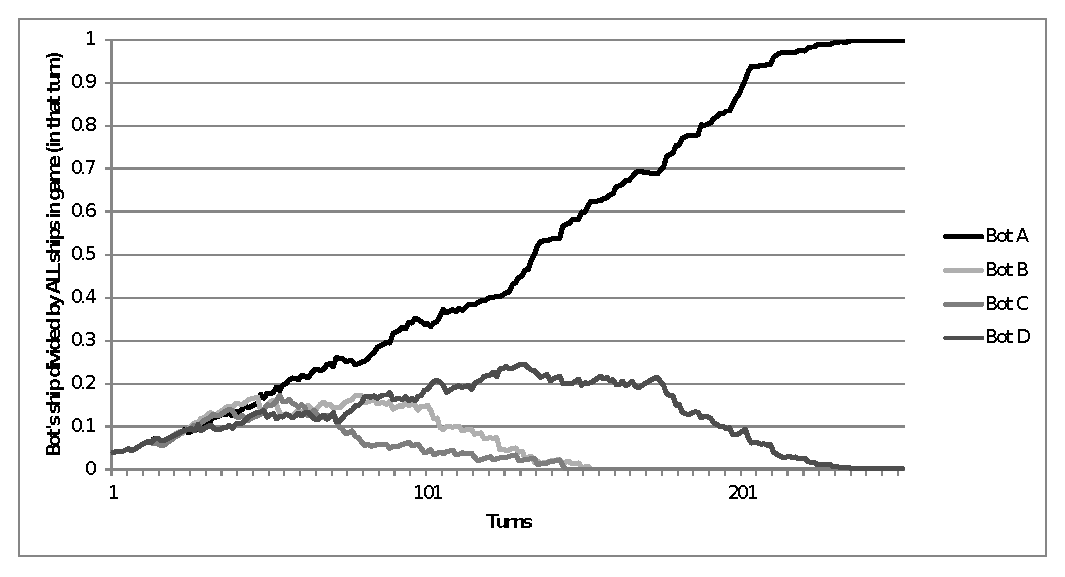
\epsfig{file=imags/nubecita.eps,width=8cm}
%\end{center}
%\caption{Representation of the number of ships of each bot in each turn} 
%\label{figura:nubecita}
%\end{figure}
Below, are described the two alternatives to deal with this cloud of points for the fitness function: the use of slopes and areas.

% ---------------------------------------------------------------------

\subsection{Fitness based in Slope}
%  "slope based fitness"   [pedro]
\label{subsec:fitness_slope}

% In this case, a square regression .......      [pedro]
In this case, a square regression analysis is computed in order to transform the cloud of points into a simple line. The line is represented as {$y = \alpha \times x + \beta $}, where {$\alpha$} and {$\beta$} are calculated as shown in Equations \ref{eq:alpha} and \ref{eq:beta}, computing a least squares regression. For every bot in the simulation we calculate $\alpha$ and ($slope$). This $slope$ is the fitness of every bot for that simulation. 

%A graphical example can be seen in Fig. \ref{figura:nubecita:pendiente}.

%%Antonio, pon esto junto si puedes, en la misma fila, que con subfigure no funciona :(
\begin{equation}
\label{eq:alpha}
        \alpha = \frac{\sum_{i=1}^{n}(X_{i} - \bar{X_{i}})(Y_{i} - \bar{Y_{i}})}{\sum_{i=1}^{n}(X_{i} - \bar{X_{i}})^{2}}
\end{equation}

\begin{equation}
\label{eq:beta}
        \beta = \bar{Y}-\alpha\bar{X}
\end{equation}


%\begin{figure}[h]
%\centering
%\hspace*{-1in}
%  \epsfig{file=imags/nubecita_pendiente.eps,width=0.6
%  \textwidth}
%\caption{Fitness based in Slope: number of ships of every bot in each turn}
%\label{figura:nubecita:pendiente}
%\end{figure}


% \begin{figure}[ht]
% \centering
% \hspace*{-1in}
% \begin{subfigure}[H]{0.4\textwidth}
% 	\large
%    \begin{equation}
%        \alpha = \frac{\sum_{i=1}^{n}(X_{i} - \bar{X_{i}})(Y_{i} - \bar{Y_{i}})}{\sum_{i=1}^{n}(X_{i} - \bar{X_{i}})^{2}}
%    \end{equation}
%    \begin{equation}
%        \beta = \bar{Y}-\alpha\bar{X}
%    \end{equation}
%    \caption{Least Squares Regression}
%    \label{equation:LeastSquares}
% \end{subfigure}
% \hfill
% \hspace*{0.2in}
% \begin{subfigure}[H]{0.7\textwidth}
% \begin{center}
%  \epsfig{file=imagenes/nubecita_pendiente.eps,width=1.1\textwidth}
% \end{center}
% \caption{Number of ships of every bot in each turn} %Maribel, cambio if por of
% \label{figura:nubecita:pendiente}
% \end{subfigure}
% \caption{Fitness based in Slope}
% \end{figure}

Theoretical maximum and minimum values are set for this fitness. An optimum bot that wins in the first turn, has an ideal slope of {$1$}, so this is the maximum value of our fitness. On the other hand, a bot that loses in the first turn,  has a slope of {$-1$}. Thus, if we calculate the $slope$, we know if the bot {$WINs$} ({$slope>0$}) or {$LOSEs$} {$slope<0$}. 
The values of the different battles are summed to compute the global $slope$. %FERGU: por qué las mayúsculas? Explicar mejor esta última frase
Then, the bot with the highest value will be the best is each turn or battle. 

%Several evaluations in different maps was using, so it's need operate with fitness. In that case, only sum the slope of all the evaluations of the bot. Maribel, esto ya lo has dicho antes y además lía más la cosa así que lo he eliminado. Además expresiones como "was using" están mal, qué quieres decir? fue usando? eso en inglés no se dice.

% ---------------------------------------------------------------------

\subsection{Fitness based in Area}
% "area based fitness"    [pedro]
\label{sec:fitness}

In this function, the integral of the curve of the bot's live-line is used for calculating the area that is `covered' by the fitness cloud of points (see Equation \ref{eq:area}). This {$area$} is normalised considering the number of turns, and thus it represents the average percentage of ships during the battle for each player. 
%An example is shown in Fig. \ref{figura:nubecita:area}.

\begin{equation}
        area=\frac{\int_{0}^{t}\%ships(x)dx}{t}
    \label{eq:area}
\end{equation}

% \begin{figure}[h]
% \begin{center}
%   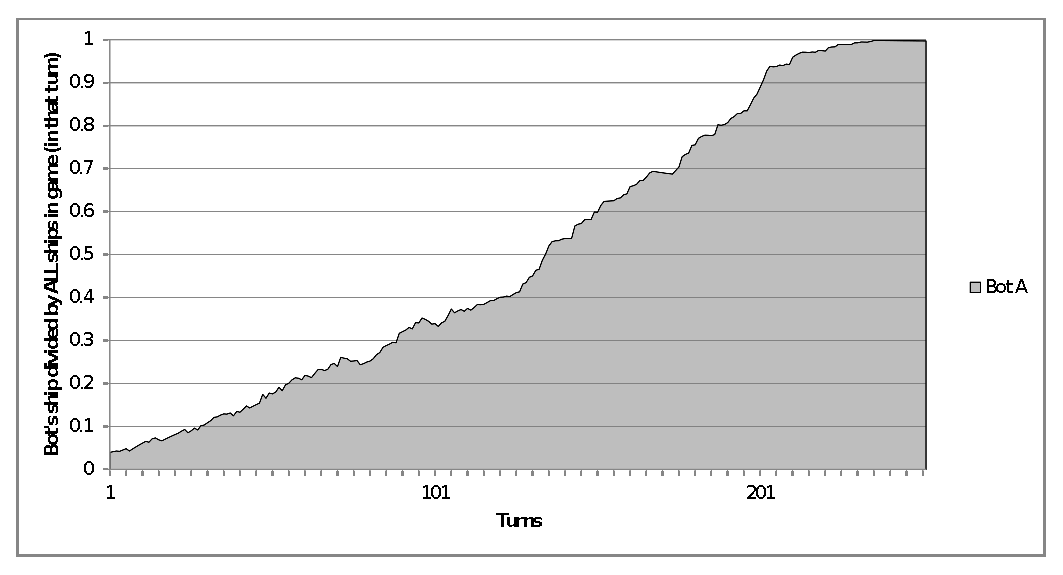
\epsfig{file=imagenes/nubecita_integral.eps,width=0.7\textwidth}
% \end{center}
% \caption{Fitness based in Area. Example of area under the live-line curve.}
% \label{figura:nubecita:area}
% \end{figure}

%\begin{figure}[h]
%\centering
%\hspace*{-1in}
%\begin{subfigure}[H]{0.4\textwidth}
%	\large
%    \begin{equation}
%        area=\frac{\int_{0}^{t}\%ships(x)dx}{t}
%    \end{equation}
%    \caption{Calculus of the area}
%    \label{equation:area}
%\end{subfigure}
%\begin{subfigure}[H]{0.6\textwidth}
%\begin{center}
%  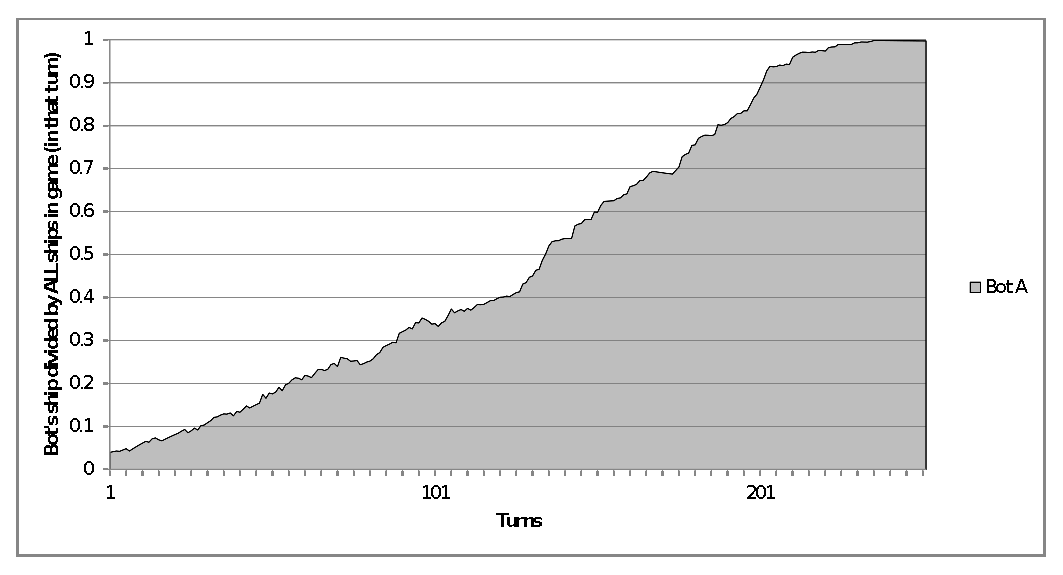
\epsfig{file=imagenes/nubecita_integral.eps,width=0.6\textwidth}
%\end{center}
%\caption{Example of area under the live-line curve.} 
%\label{figura:nubecita:area}
%\end{subfigure}
%\caption{Fitness based in Area}
%\end{figure}

As in previous case, maximum and minimum values has been set for this fitness. If an optimal bot wins in the first turn, the area of each live-line is close to {$1$}, so this is the maximum value of the fitness. Otherwise, if a bot loses in the first turn, its live-line area is close to {$0$}. In this case, we do not extract additional about which bot wins the battle, because the area of the live-line is not related with the winner of the battle. Thus, we are losing some information. 
%FERGU: y por lo tanto... blablabla. No usar el we.
% AntonioDEF - completar esto (ANTARES escribe y FERGU revisa) :D

%-----------------------------------------------------------------------
%%%%%%%%%%%%%%%%%%%%%%%% EXPERIMENTAL SETUP %%%%%%%%%%%%%%%%%%%%%%%%%%%%
%-----------------------------------------------------------------------

\section{Experimental Setup}
\label{sec:experiments}

% in order to ensure a fair comparison of the three fitness functions
% we have decided to compare an equal number of evaluations - equal
% time what??? - JJ
Sub-tree crossover and 1-node mutation evolutionary operators have
been used, following other researchers' proposals that have used these
operators obtaining good results \cite{Esparcia2013GPunreal}. In this
case, the mutation randomly changes the decision of a node or mutate
the value with a step-size of 0.25 (an adequate value empirically
tested). Each configuration is executed 30 times, with a population of
32 individuals and a 2-tournament selector for a pool of 16
parents.

%This is not experimental setup, it is description of
%parameters used in the algorithm. Experimental setup is
%number of runs, which conditions, so on - JJ

To test each individual during the evolution, a battle with a previously created bot is performed in 5 different (but representative) maps provided by Google is played. 
%Hierarchical fitness is used, as proposed in \cite{Genebot_CEC11}. Thus, an individual is better than another if it wins in a higher number of maps. In case of equality of victories, then the individual with more turns to be defeated (i.e. the stronger one) is considered better. The maximum fitness is, therefore 5 victories and 0 turns. 
Also, as proposed by \cite{Genebot_CEC11}, and due to the fact that
different evaluations will yield different values, all individuals are
re-evaluated in every generation, constituting an implicit averaging
 \cite{Jin2005303,DBLP:conf/ijcci/MereloLFGCCRMG15}.
% 1. You could cite our papers on noise
% 2. You could USE the conclusions of those papers. In this case: ?use
% all evaluations in all generations! - JJ


A publicly available bot has been chosen for our experiments\footnote{It can be downloaded from \url{https://github.com/deantares/genebot}}. The bot to confront is {\em GeneBot}, proposed in \cite{Genebot_CEC11}. As stated, this bot was trained using a GA to optimise the 8 parameters that conforms a set of hand-made rules, obtained from an expert human player experience.  Table \ref{tab:parameters} summarises all the parameters used.

\begin{table}
\begin{center}
\begin{tabular}{|c|c|}
\hline
{\em Parameter Name} & {\em Value} \\\hline \hline
Population size & 32 \\\hline
Crossover type & Sub-tree crossover \\ \hline
Crossover rate & 0.5\\ \hline
Mutation  & 1-node mutation\\ \hline
Mutation step-size & 0.25 \\ \hline
Selection & 2-tournament \\ \hline
Replacement & Steady-state\\ \hline
Stop criterion & 50 generations \\ \hline
Maximum Tree Depth & 7  \\ \hline %FERGU: quitados distintos tamaños
Runs per configuration & 30 \\ \hline
Evaluation & Playing versus GeneBot \cite{Genebot_CEC11}  \\ \hline 
%FERGU: Antares, confirmalo
% Antonio - Al final creo que sólo Genebot %FERGU2: quitado
% Antares: Si
Maps used in each evaluation & map76, map69, map7, map11, map26 
% AntonioDEF - los mapas han sido esos, ¿no?
% Antares: Si
\\ \hline
\end{tabular}
\caption{Parameters used in the experiments.}
\label{tab:parameters}
\end{center}
\end{table}

% ¿cómo se han obtenido los valores de esos parámetros?   [pedro]
% AntonioDEF - habla un poco de los parámetros Fergu. Dí que se ahn obtenido por systematic experimentation y justifica la profundidad de 7, pero sin decir nada del artículo del EVO*. XD
% que es un valor habitual, que dado el número de antecedentes es un valor justo, no sé...
 

After all the executions we have evaluated the obtained best individuals in all runs confronting to the other bots in a larger set of maps to study the behaviour of the algorithm and how good are the obtained bots versus enemies and maps that have not been used for training.

%FERGU3: ANTARES, confirma como has hecho esto ANTARES: Confirmo, se ha hecho la prueba en 4 mapas adicionales desconocidos y frente a oponentes desconocidos a su vez (los que han generado los métodos)


The used framework is OSGiLiath, a service-oriented evolutionary framework. %\cite{Garcia13Service}. 
The generated tree is compiled in real-time and injected in the agent's code using Javassist \footnote{\url{www.javassist.org}} library. All the source code used in this work is available under a LGPL V3 License in \url{http://www.osgiliath.org}.


%-------------------------------------------------------------
%%%%%%%%%%%%%%%%%%%%%%%% RESULTS %%%%%%%%%%%%%%%%%%%%%%%%%%%%%
%-------------------------------------------------------------
\section{Results}
\label{sec:results}
\subsection{-- EA --}

Table \ref{tab:results3config} shows the obtained results after
executing each approach 21 times, i.e. GP algorithm using every fitness implementation. 
% AntonioDEF - aclaro un poco más
% la frase está mal construida después de i. e. - JJ
Although these fitness are not comparable, as they obviously apply different metrics, the \textit{Victory-based} fitness achieves values near to the optimum (5) at the end of the run (look at the best individual and average population values). The \textit{Slope} and \textit{Area} fitness yield results under their theoretical optimum, 
% AntonioDEF - ¿cuál es su óptimo teórico?
% Antares: Esto ya lo he comentado varias veces, todos tienen como rango de valores entre 0 y 5.
as they depend on more information ranges (variation in the number of ships).
\textit{Area} obtains slightly better values than \textit{Slope}. 
%Fig.\ref{fig:evolutionFitness} shows how --TO DO COMENTADO-- %Básicamente quiero decir que en la figura 2 se muestra como el fitness del mejor individuo de la población mejora a medida que transcurren las generaciones, que es lo que debe suceder en un EA. De igual manera, la figura 3 muestra como el promedio de la población también mejora a medida que van transcurriendo las generaciones.

%La figura 4 muestra el tamaño del árbol de los mejores individuos de cada generación. Los tres métodos de fitness estudiados producen árboles cada vez más grandes (o complejos) en las sucesivas generaciones. El fitness basado en victorias es el que menor crecimiento tiene, llegando a tener árboles de poco tamaño que aún así consiguen ser el mejor individuo de la población.

%La figura 5 muestra la antiguedad promedida de la población durante cada generación de todas las ejecuciones de cada método. Un crecimiento constante indicaría que la población es cada vez más vieja, por lo que no se están produciendo reemplazamos de nuevos individuos. Esto indicaría que no se están generando nuevos individuos con fitness mejores a los de sus ancentros. En los tres métodos estudiados, no se aprecia un crecimiento constante, por lo que el algoritmo está generando nuevos individuos que superan a sus padres constantemente. Los individuos están de media 4-5 generaciones antes de ser sacados del pool de la población reemplazados por individuos mejores que ellos.

% NI IDEA PORQUE NO LOS ENTIENDO XDD (FERGU3). ARREGLADLO
% AntonioDEF - yo tampoco sabría justificarlo. ANTARES dí algo y lo traduce Fergu. ;D

% ANTARES: Cómo he re-ajustado las figuras para hacer comparaciones "entre mismo tipos de fitness" ha cambiado un poco las gráficas.
% las gráficas de convergencia del algoritmo sirven para demostrar que realmente el algoritmo esta convergiendo hacia mejores soluciones según el fitness.


\begin{figure}[ht]
 \begin{center}
   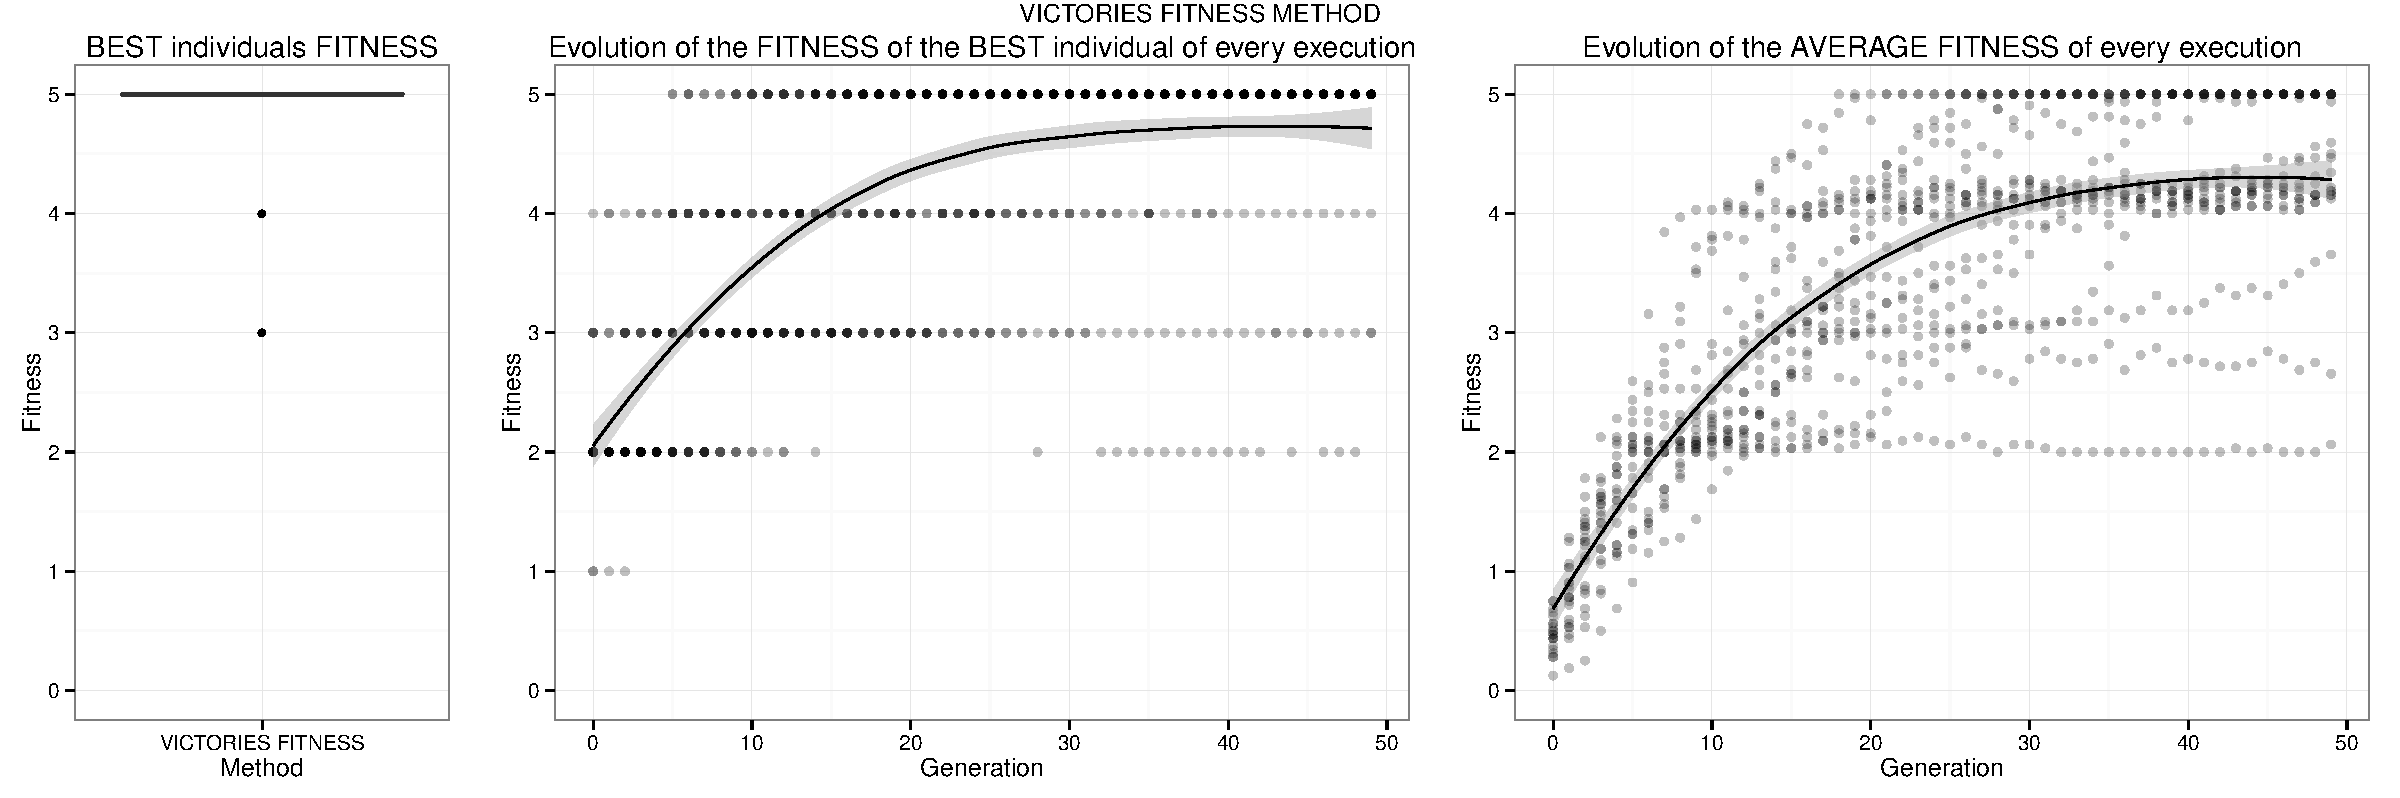
\includegraphics[width=12cm]{nuevas_imgs/estudio_turns.pdf}
 \end{center} % no podéis empezar una frase con "for
              % individuals". Empezad con Boxplot - JJ También es
              % inútil un boxplot sólo, sólo sirve para comparar. - JJ
 \caption{\textbf{Victories Fitness Method} individuals: Boxplot of the fitness of the \emph{Best individuals} of every execution and evolution of the \emph{Best fitness} and \emph{Average population fitness} of every execution. In evolution plots, single points and locally weighted polynomial curve (loess) are shown.}
 \label{figura:fitness_turns}
 \end{figure}

   \begin{figure}[ht]
 \begin{center}
   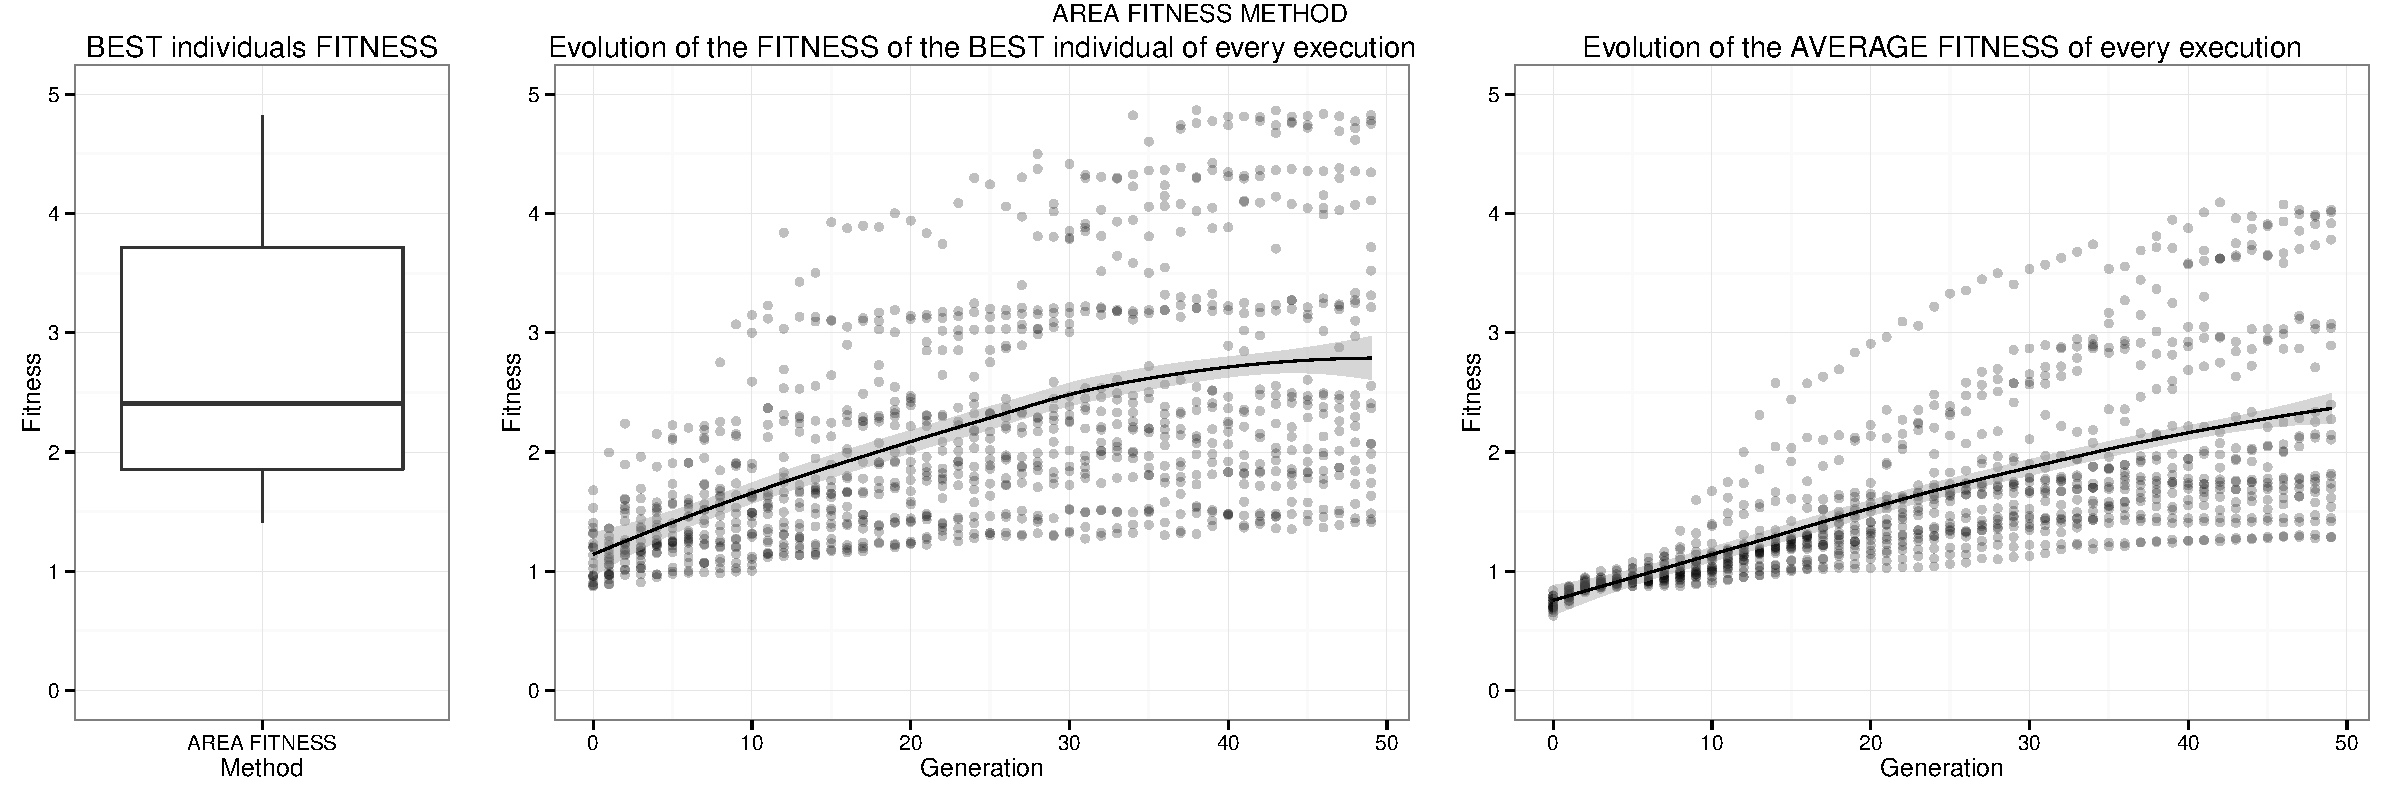
\includegraphics[width=12cm]{nuevas_imgs/estudio_area.pdf}
 \end{center}
 \caption{\textbf{Area Fitness Method} individuals: Boxplot of the fitness of the \emph{Best individuals} of every execution and evolution of the \emph{Best fitness} and \emph{Average population fitness} of every execution. In evolution plots, single points and locally weighted polynomial curve (loess) are shown.}
 \label{figura:fitness_area}
 \end{figure}

    \begin{figure}[ht]
 \begin{center}
   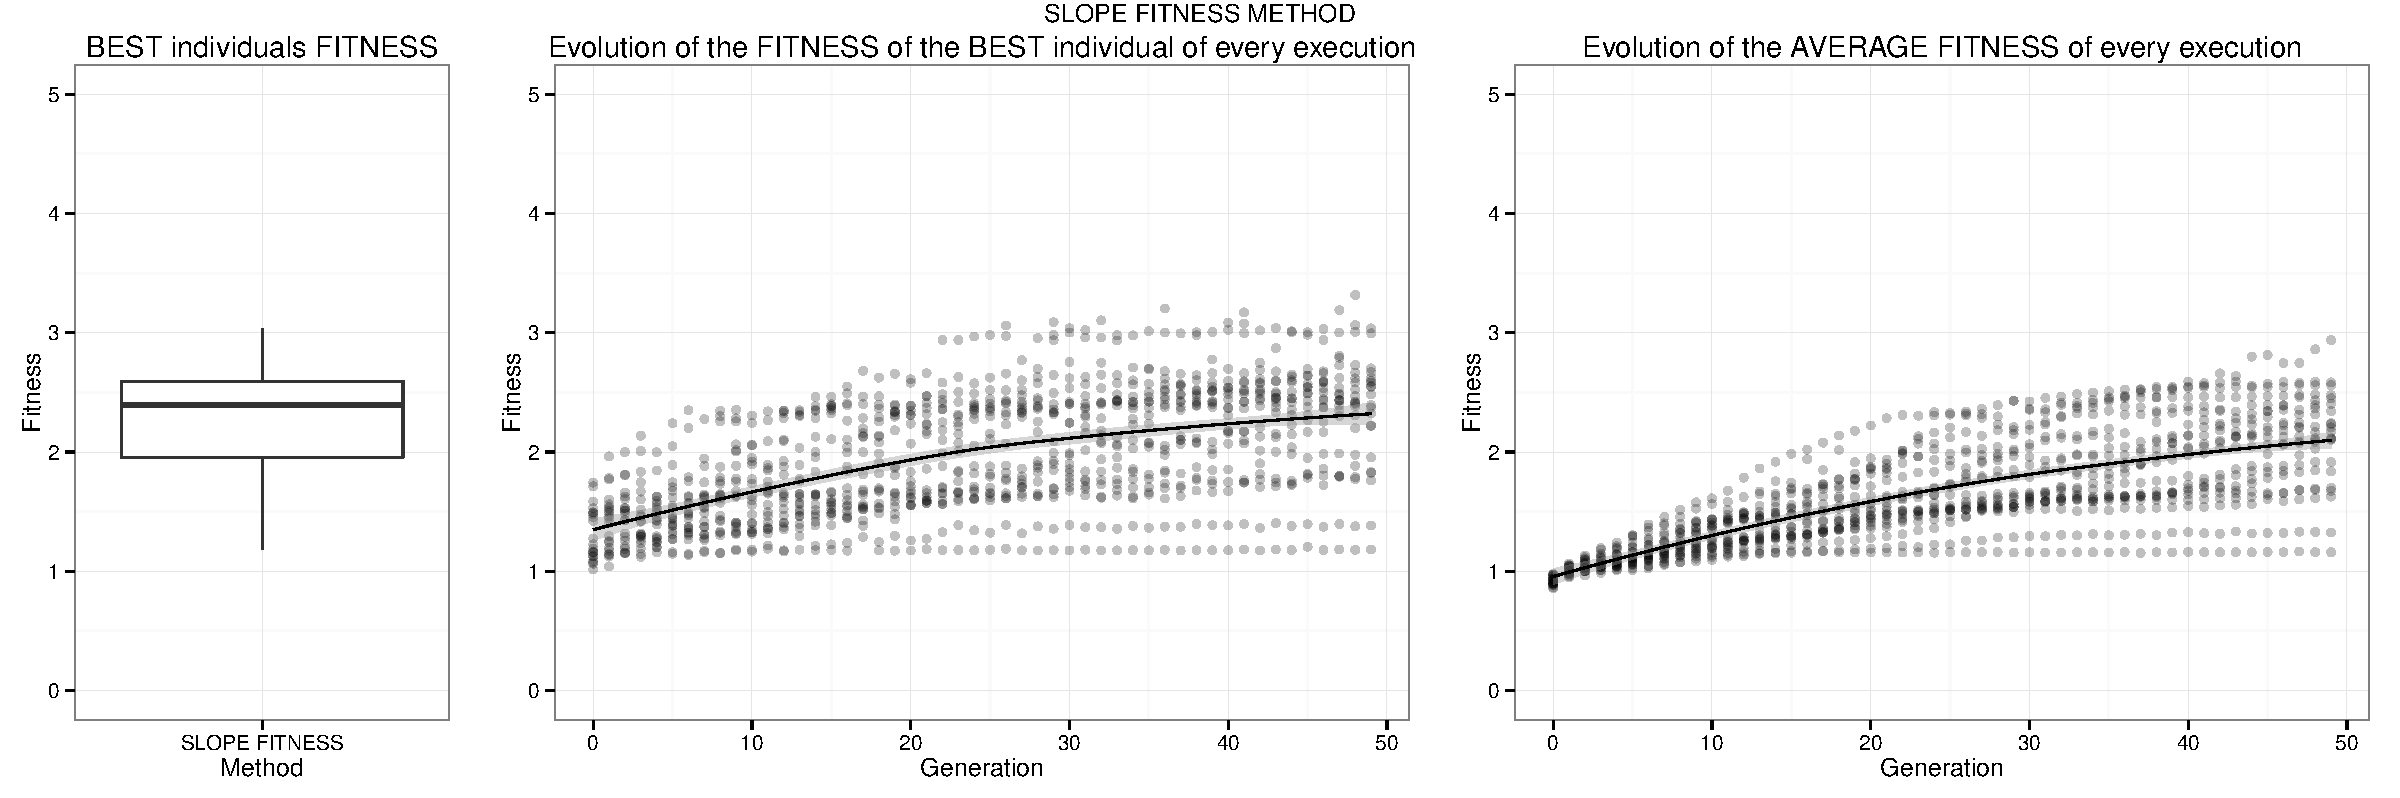
\includegraphics[width=12cm]{nuevas_imgs/estudio_slope.pdf}
 \end{center}
 \caption{\textbf{Slope Fitness Method} individuals: Boxplot of the fitness of the \emph{Best individuals} of every execution and evolution of the \emph{Best fitness} and \emph{Average population fitness} of every execution. In evolution plots, single points and locally weighted polynomial curve (loess) are shown.}
 \label{figura:e_fitness_slope}
 \end{figure}


 % \begin{figure}[ht]
 % \begin{center}
 %   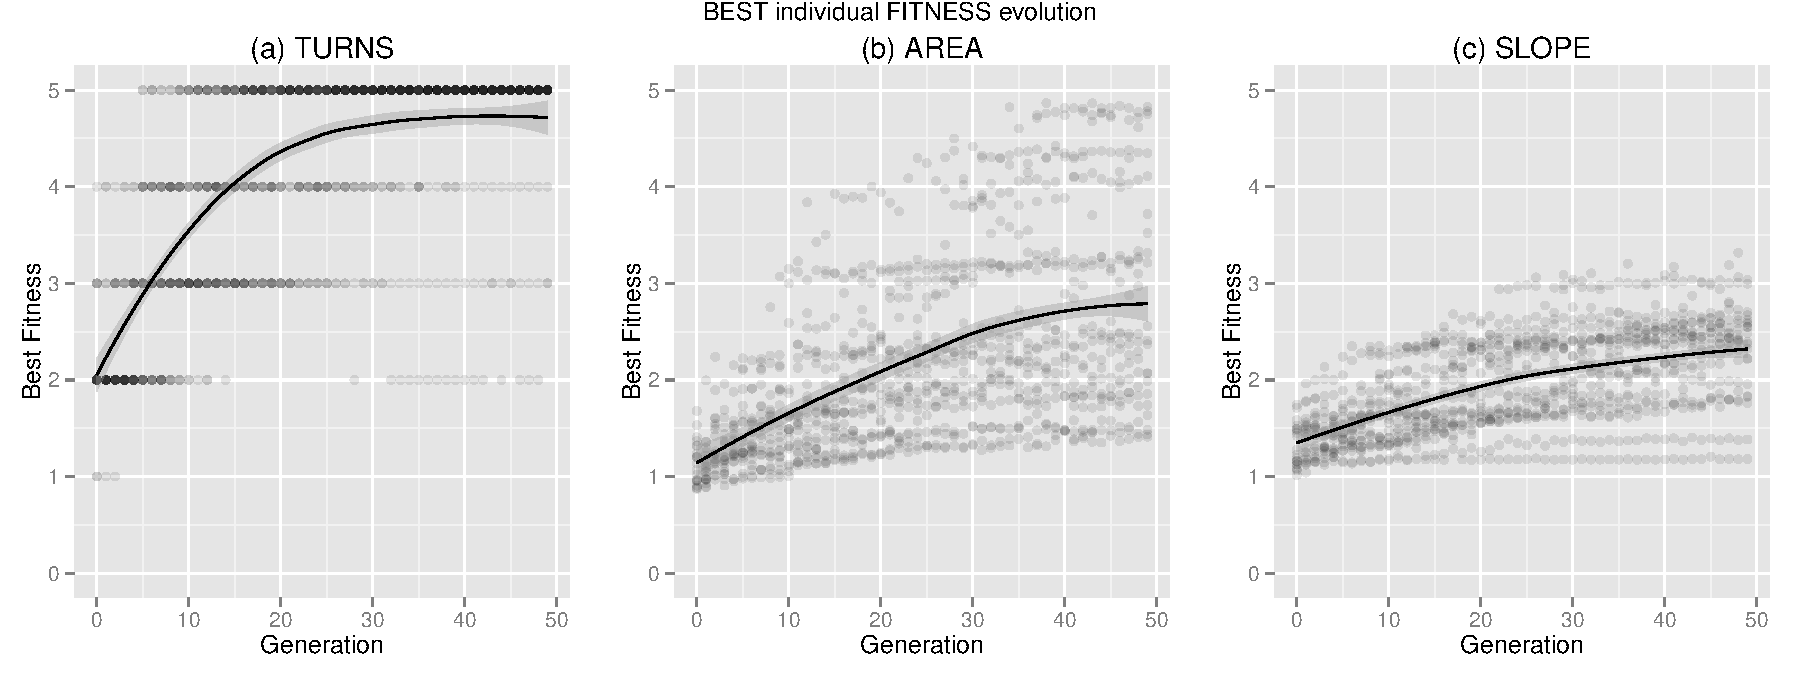
\includegraphics[width=12cm]{nuevas_imgs/evolution_BEST_FITNESS.pdf}
 % \end{center}
 % \caption{Evolution of the fitness of the best individual of every execution by fitness method.}
 % \label{fig:evolutionFitness}
 % \end{figure}

 % \begin{figure}[ht]
 % \begin{center}
 %   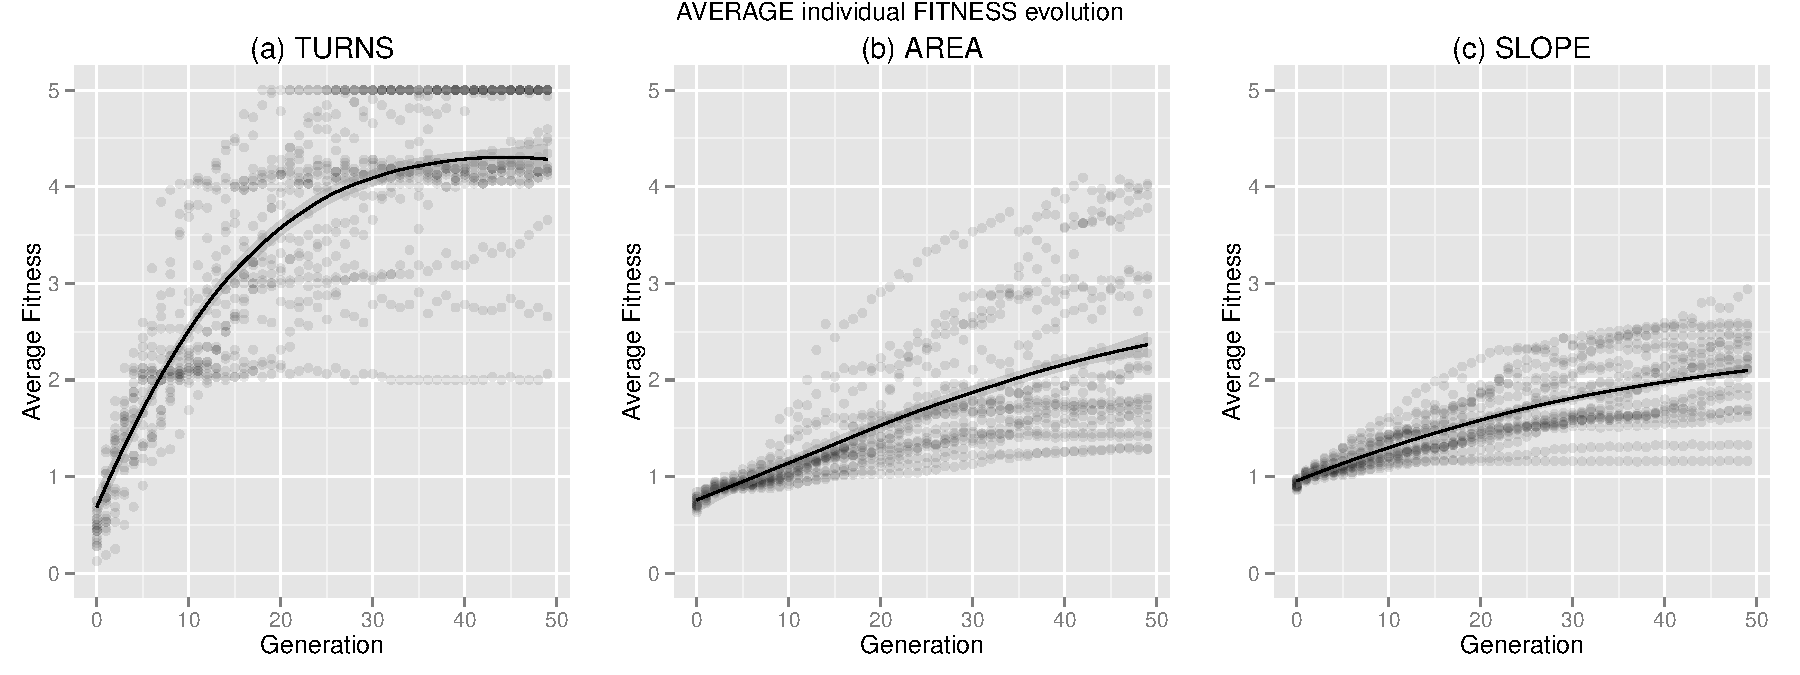
\includegraphics[width=12cm]{nuevas_imgs/evolution_AVERAGE_FITNESS.pdf}
 % \end{center}
 % \caption{Evolution of the average fitness of every execution by fitness method.}
 % \label{figura:evolutionFitnessAverage}
 % \end{figure}

 \begin{figure}[ht]
 \begin{center}
   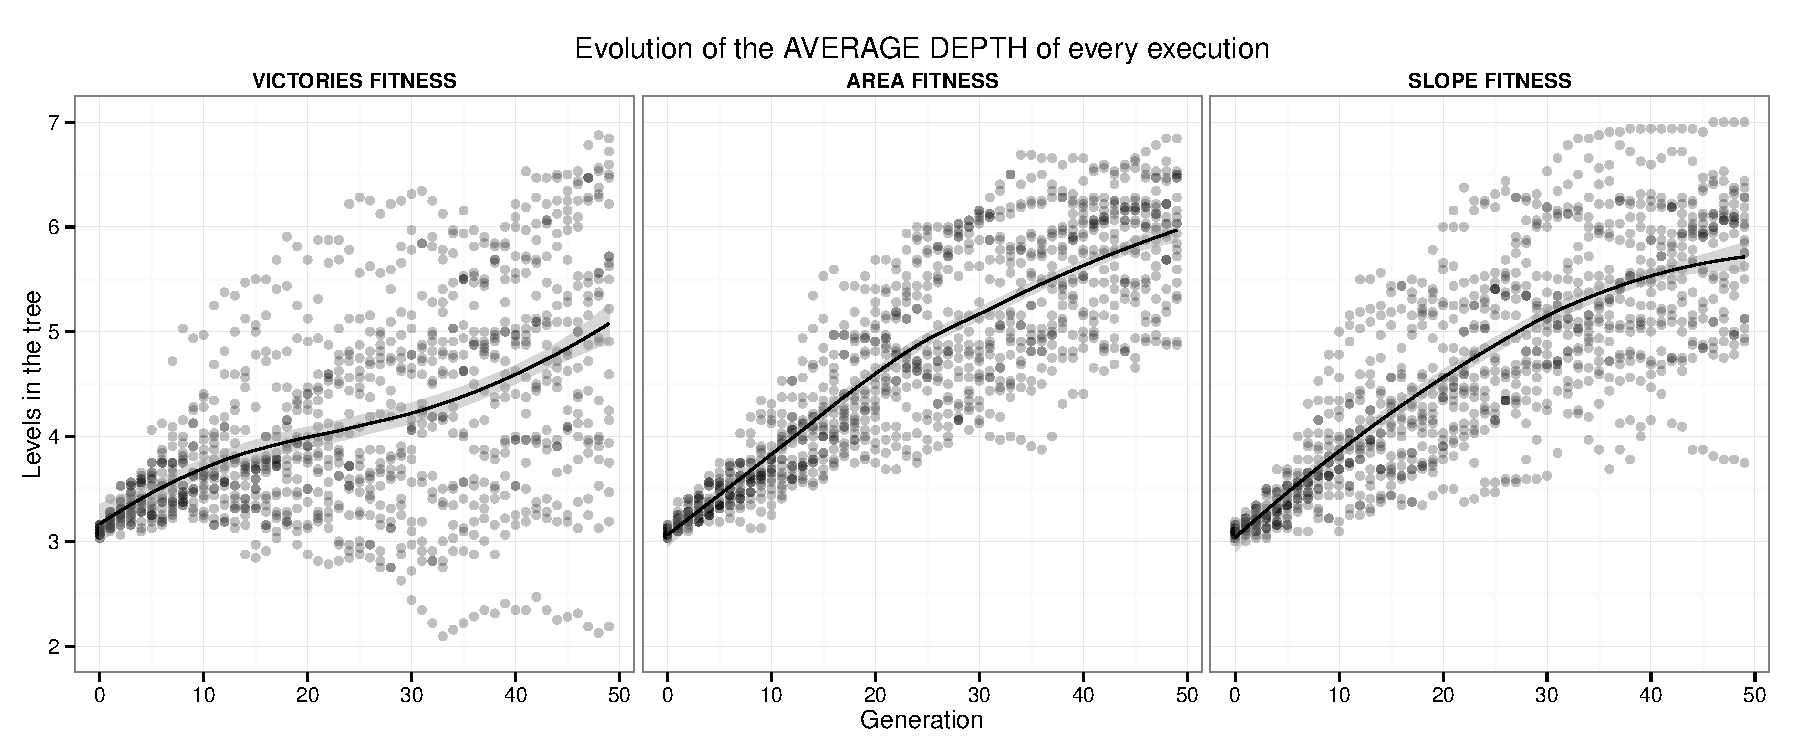
\includegraphics[width=12cm]{nuevas_imgs/evolution_AVERAGE_DEPTH.pdf}
 \end{center}
 \caption{Evolution of the average depth of every exectuion by fitness
   method. -- TO DO --} % What is this for? - JJ
 \label{figura:evolutionDEPTH}
 \end{figure}

 \begin{figure}[ht]
 \begin{center}
   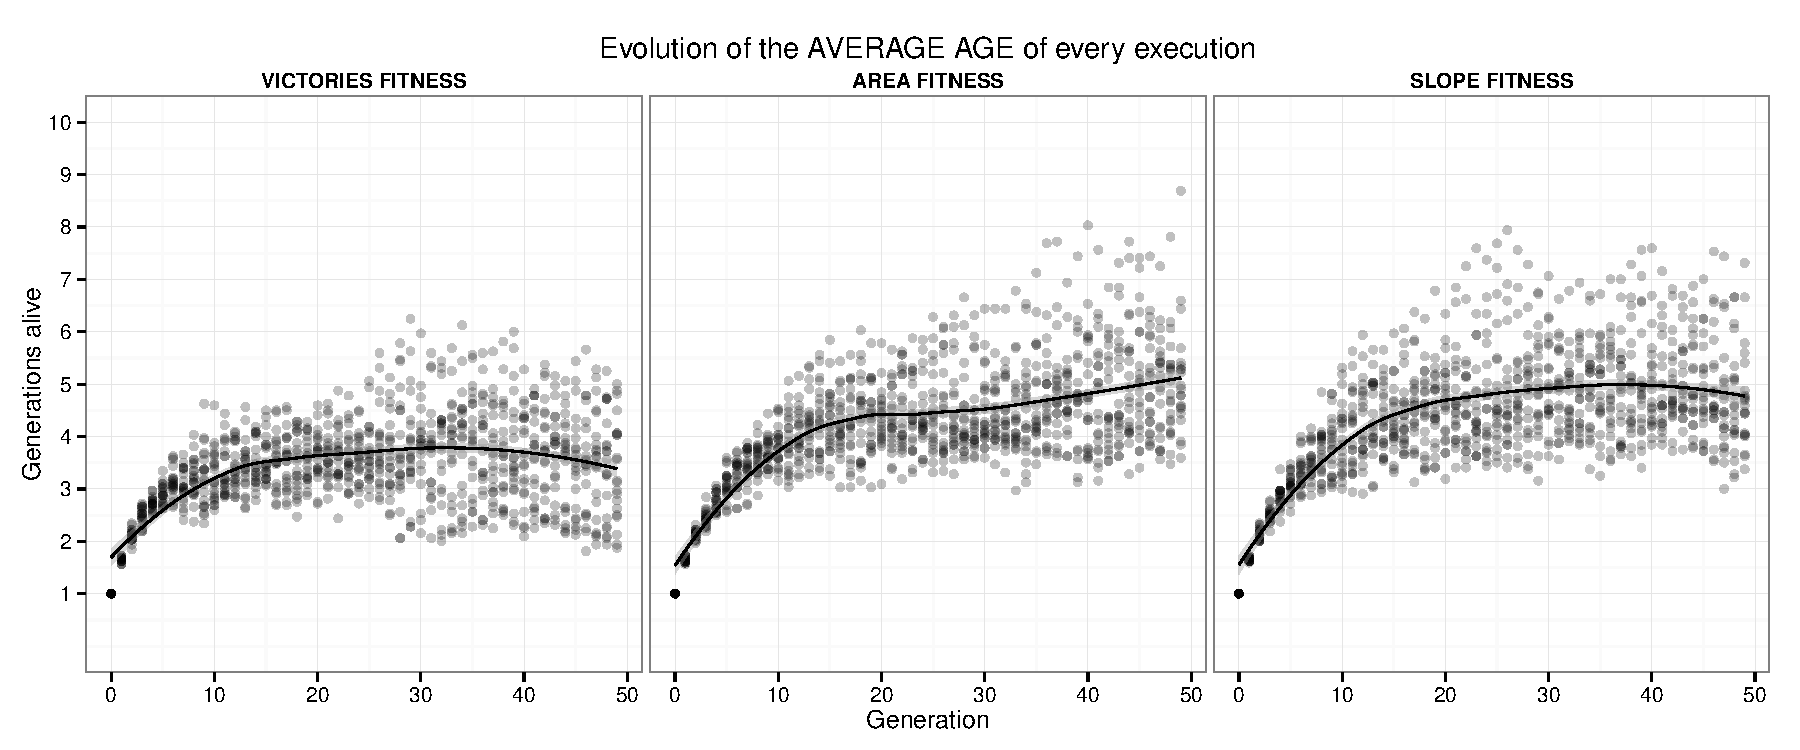
\includegraphics[width=12cm]{nuevas_imgs/evolution_AVERAGE_AGE.pdf}
 \end{center}
 \caption{Evolution of the average age of every execution by fitness
   method. -- TO DO -- Un crecimiento constante de la edad indicar?
   que el algoritmo no est?generando individuos que sean mejores que
   los anteriores, por lo que se habr? ...} %don't use Spanish!!!!! 
% Where did you see that method of evaluating different fitness
% functions? - JJ
 \label{figura:evolutionAGE}
 \end{figure}

\begin{table*}
\centering{
\begin{tabular}{|c|c|c|} \hline            
		& Average best fitness	&	Average population fitness	\\ \hline \hline
Victory	& 4,761 $\pm$	0,624	&	4,345	$\pm$	0,78 \\ \hline
Slope	& 2,296	$\pm$	0,486	&	2,103	$\pm$	0,434 \\ \hline
% AntonioDEF - la misma desv. típica? huele a copy-paste mal hecho. XD
% Antares: Comprobado, había un error en el copy paste, corregido.
Area	& 2,838	$\pm$	1,198	&	2,347	$\pm$	0,949 \\ \hline


\end{tabular}
\caption{Average results obtained for each approach at the end of the
  runs. Everyone has been tested 21 times.}
%Don't understand this. How do you compare fitnesses if they are
%computed in a different way? Shouldn't you call it score? Or
%victories? Or something else? - JJ
% ANTARES: See next section ;)
\label{tab:results3config}
}
\end{table*}

\subsection{-- TO DO -- Fitness Benchmark}

Even though the \textit{Victory-based} fitness yields better results
(near optimal), to do a fair comparison, we have confronted the 21
best bots obtained with each configuration (one per run) against
GeneBot. However these matches have been performed in 9 maps that were
different to the ones used to evolve the bots. These % cuales? Los 9?
                                % - JJ
maps, provided by Google, are considered as representative, because they have different features to promote a wide set of strategies, i.e. different distributions of planets, sizes and number of initial ships. 

This experiment has been conducted in order to validate if the bots obtained by the proposed approaches can be competitive in terms of quality in maps not used for evolution/evaluation. Results are shown in Figure \ref{figura:boxplotvictoriesgenebot}. As it can be seen, again the \textit{Victory-based} fitness achieves significantly better results than the other methods.


\begin{figure}[ht]
 \begin{center}
   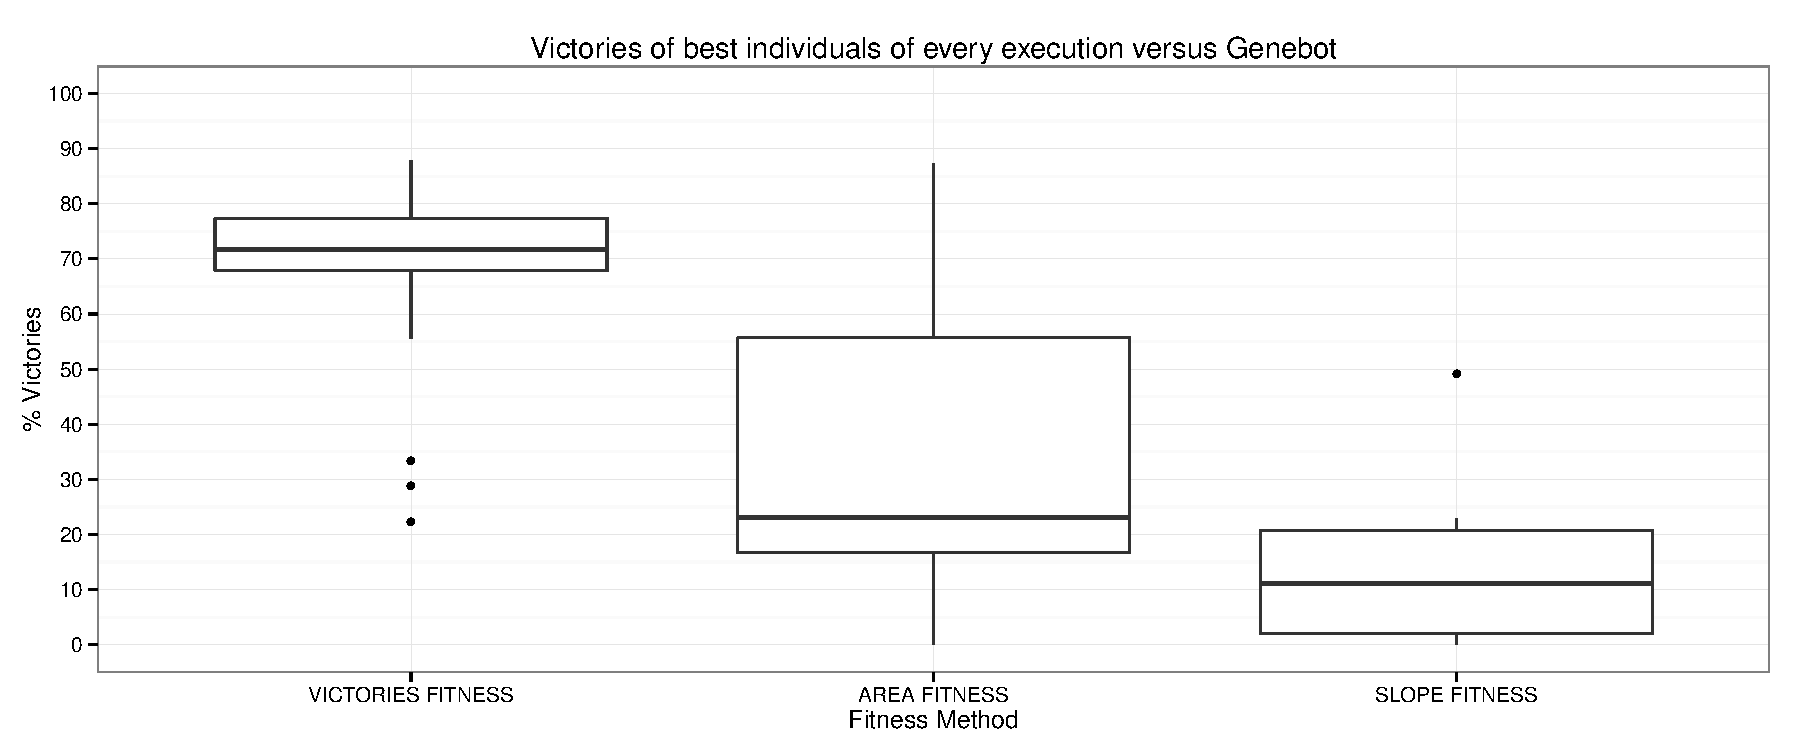
\includegraphics[width=12cm]{nuevas_imgs/vsGENEBOT_Boxplot.pdf}
 \end{center}
 \caption{Boxplot of average percentage of victories of the bots obtained by each approach vs. GeneBot. 9 different matches have been performed per bot in different maps.} 
% AntonioDEF - ¿average percentage o sólo percentage? (ANTARES)
% Toy un poco dormío ya para pensar. :/
% Antares: No, a ver. Se coge cada individuo y se le evalúa contra Genebot. Ese gana pues digamos un 90%. Se coge otro y se prueba, gana el 70%.... Con todos esos valores se hace un bloxplot. Así que no es el promedio.
 \label{figura:boxplotvictoriesgenebot}
 \end{figure}

Finally, an additional experiment has been conducted, proposing a direct comparison between the three methods. To this end each of the best individuals obtained per approach has been tested competing against all the rest (in a vs 1 battles) in 9 matches per pair of bots, one per representative map.
% AntonioDEF - ¿en cuantos mapas? o sea, ¿cuántos combates hacía cada pareja?
% revisad si está bien así. (ANTARES).
% Antares: Está explicdo más adelante

This allows a comparison with a bigger number of bots, and also,
allows the analysis of their behaviour against rivals not previously
used during training (as in the experiment above). 
The boxplots of the average percentage of victories from the best bots obtained by each method are shown in Figure \ref{figura:boxplotvictories}. It is clear from the image that the \textit{Slope} fitness does not get good results with respect to the other methods. This can be explained because the this fitness loses information during the run, in comparison with the others, obtaining bots less aggressive. 
% AntonioDEF - ¿Qué información pierde?¿Esto de dónde os lo habeis sacado?¿Cómo lo sabéis? (ANTARES)
% Antares: Yo no he sacado ese texto. Supongo que lo querrá decir, es que el fitness basado en pendiente suma puntos si gana (la pendiente es positiva) o resta si pierde (la pendiente es negativa). Así que supongo que lo que se quiere decir es que la puntuación no se sabe cuanto ha sumado y cuando ha restado. Igual a sumado mucho pero ha restado algo. O igual ha sumado muy poco. No sé a que otra cosa se puede referir.
The \textit{Victory-based} fitness achieves better results in average, being also more robust (small standard deviation). However, looking at the \textit{Area} fitness results, they outperform several times the \textit{Victory} results, obtaining more victories.
%.... NO SE COMO JUSTIFICAR QUE ESTO ES MEJOR :/// (FERGU3). ç

%FERGU3 ANTARES, CUANTAS EJECUCIONES POR BOT Y EN QUE MAPAS?????  
%Los mapas son & 7 & 11 & 13 & 26 & 32 & 64 & 69 & 76 & 87 \ y os explico un poco las cuentas.
%Se han hecho 35721 batallas en 9 mapas con 63 bots (21 por método).
%Cada bot se ha enfrentado con los otros bots en 9 mapas (63 enfrentamientos) más luego él mismo ha servido como rival para los otros bots (otros 63 combates)
% AntonioDEF - esto supongo que es de aquí

 \begin{figure}[ht]
 \begin{center}
   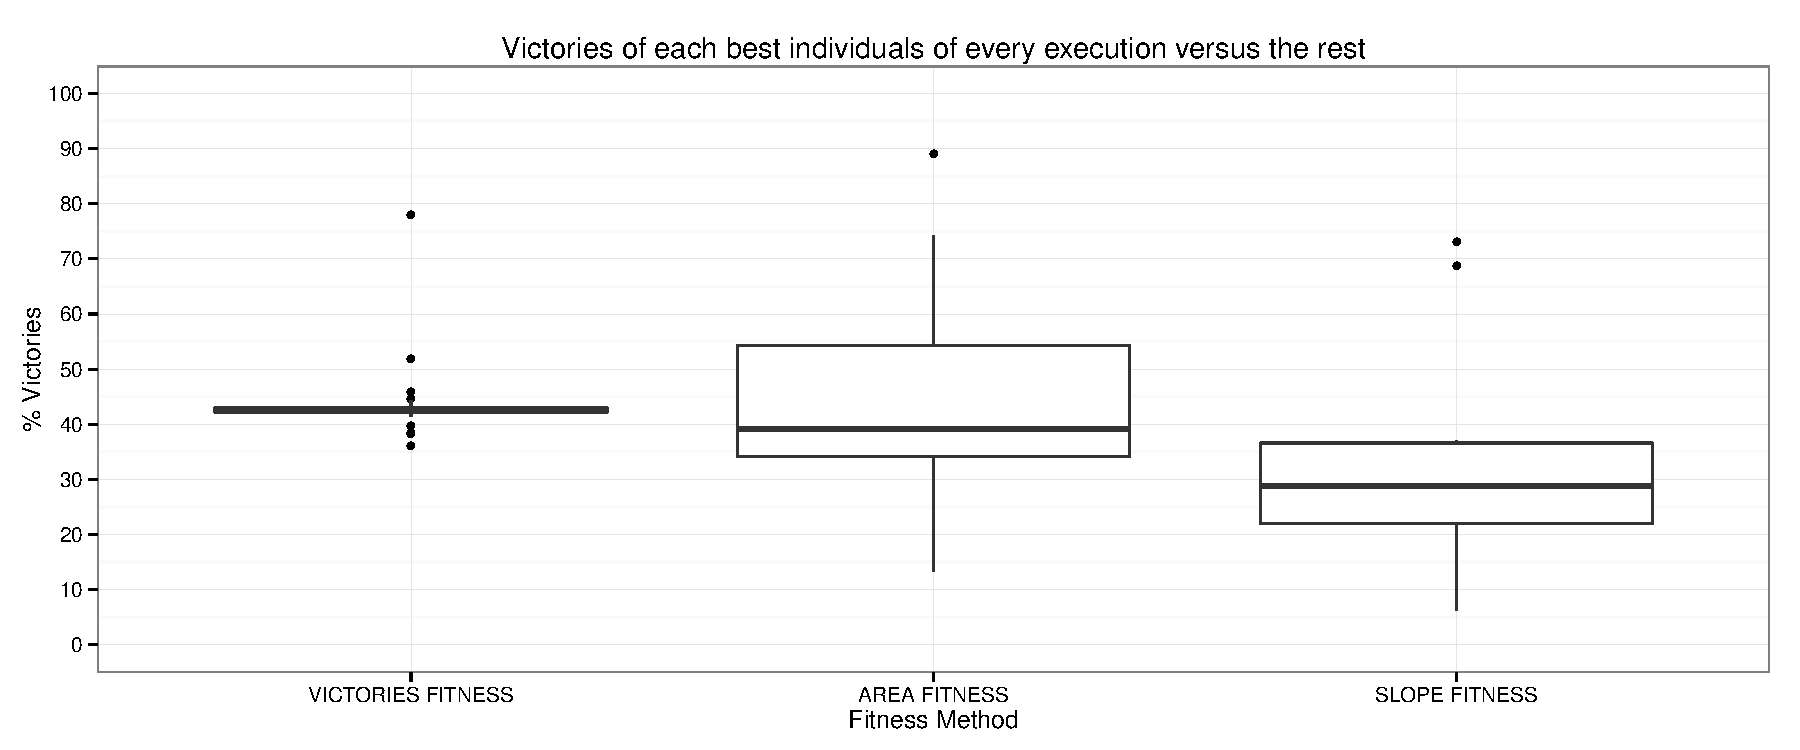
\includegraphics[width=12cm]{nuevas_imgs/batallas_Boxplot.pdf}
 \end{center}
 \caption{Boxplot of average percentage of victories of the best bots obtained by each method vs. the rest.}
% Los boxplot son para comparar. Los tenéis que meter a los tres en el mismo. Si no vais a comparar, no tenéis que hacer ningún boxplot. - JJ FERGU4: lo que te dije, Antares. 
% Antares: a ver, aquí si se comparan la misma cosa, el porcentaje de
% victorias de cada individuo. En principio en el texto hay que
% compararlos.
% Por favor, corregid el título de los gráficos "victories of best"
% está mal dicho. Ponedlo consistente en todos los gráficos también. 
 \label{figura:boxplotvictories}
 \end{figure}


There is still a final remark, which concerns to the percentage of draw matches.

%As it can be seen in Table \ref{tab:ties}. The matches with bots obtained using \textit{Victory-based}
%fitness  result in more ties against bots of the same type than the
%other approaches. % so what? - JJ

This can be explained because they use less
information to perform the evolution, obtaining quite similar
behaviours. % which is good because a) it is more consistent b) more
            % robust c) no idea - JJ
This is also reinforced by previous results in which the
bots of this fitness seemed to perform similarly, obtaining close
number of victories and thus, getting small standard deviation
values. 
% AntonioDEF - a ver si os mola esta conclusión. (ANTARES)
% Don't understand a thing. Which one is better? Why do you use the
% number of ties to compare them? Shouldn't you compare the number of
% ties _with itself_ with the number of ties _with the best bots
% created with other methods? - JJ


% \begin{table*}
% \centering{
% \begin{tabular}{|c|c|c|c|} \hline            
% 		& Victory		&	Area 		& Slope	\\ \hline \hline
% Victory & 62.06\%	& 23.15 \% 	&	12.47 \% \\ \hline
% Slope	& 	-		& 19.07 \%	&	12.50 \%		\\ \hline
% Area	& 	-		&	-		&	11.87 \% \\ \hline

% %This table is WRONG!!! They are not in the same order. Area vs. Area,
% %for instance is not completed - JJ
% %  \begin{table}[ht]
% % \centering
% % \begin{tabular}{rlr}
% %   \hline
% %  FITNESS METHOD & Victories\\ 
% %   \hline
% %  VICTORIES FITNESS & 68.04\% \\ 
% %  AREA FITNESS & 33.01\% \\ 
% %  SLOPE FITNESS & 13.17\% \\ 
% %    \hline
% % \end{tabular}
% %  \caption{ -- TO DO -- Victories vs Genebot}
% %  \label{tabla:vsGenebot}
% % \end{table}


% \end{tabular}
% \caption{Percentage of draw matches between bots per fitness approach.}
% \label{tab:ties}
% }
% \end{table*}

% Antares: esta tabla se va fuera, porque estoy intentando hacerlo de otra manera y ahora mismo no aporta mucho, para que decir lo contrario.

\subsection{-- TO DO -- Estudio acciones y condiciones}

 \begin{figure}[ht]
 \begin{center}
   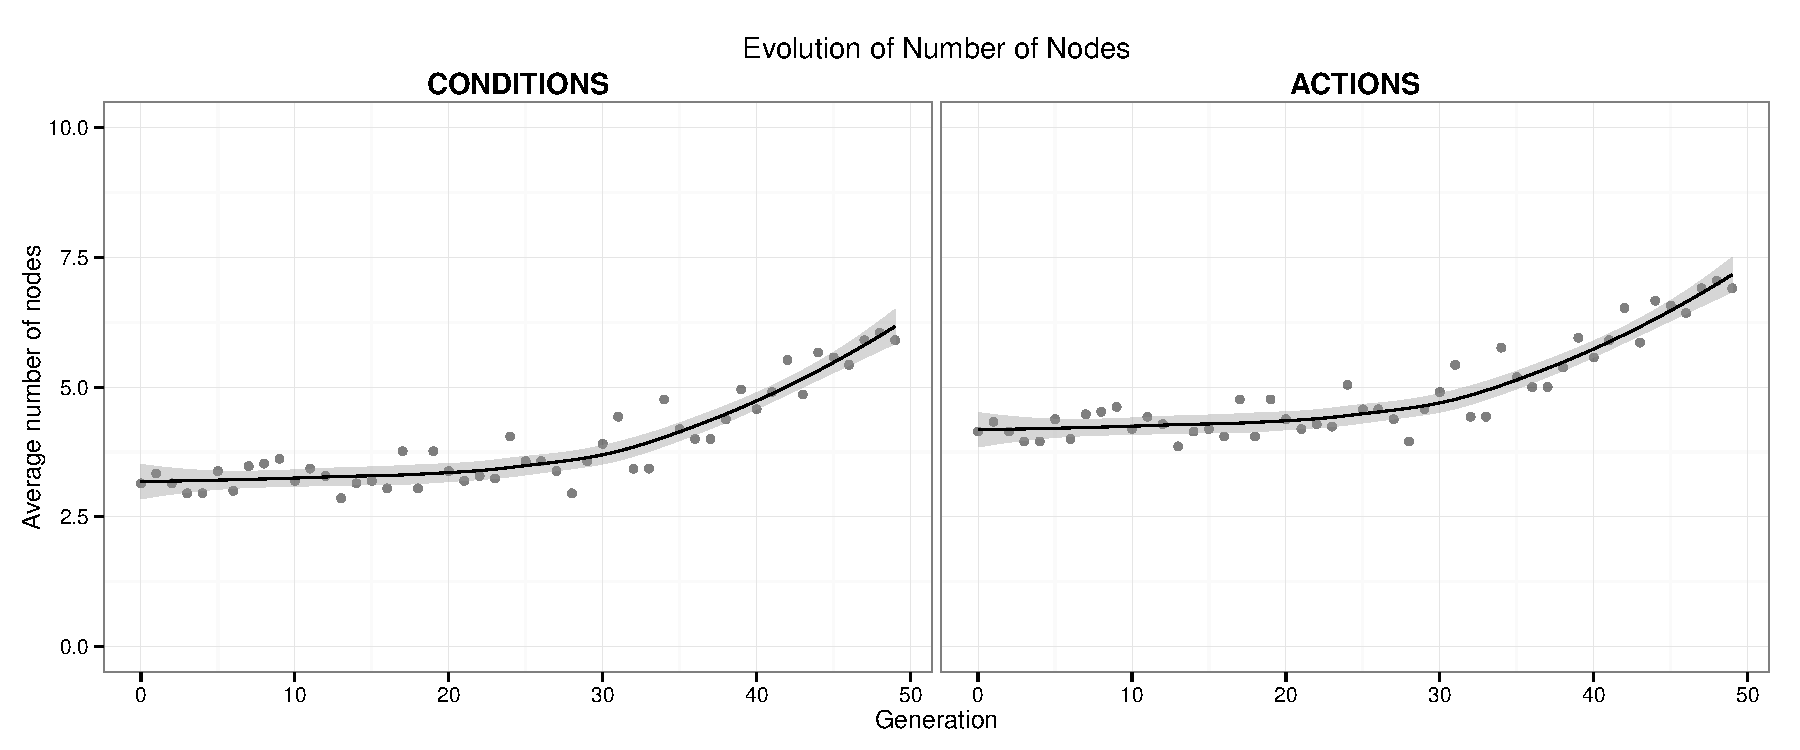
\includegraphics[width=12cm]{nuevas_imgs/estudio_number_nodes.pdf}
 \end{center}
 \caption{Evolution of the number of nodes of the best individual by generation of every execution. Nodes can be conditions (internal nodes) or actions (lead nodes). The tree is always a binary tree, so both (conditions and actions) are related.}
 \label{figura:e_number_nodes}
 \end{figure}

 \begin{figure}[ht]
 \begin{center}
   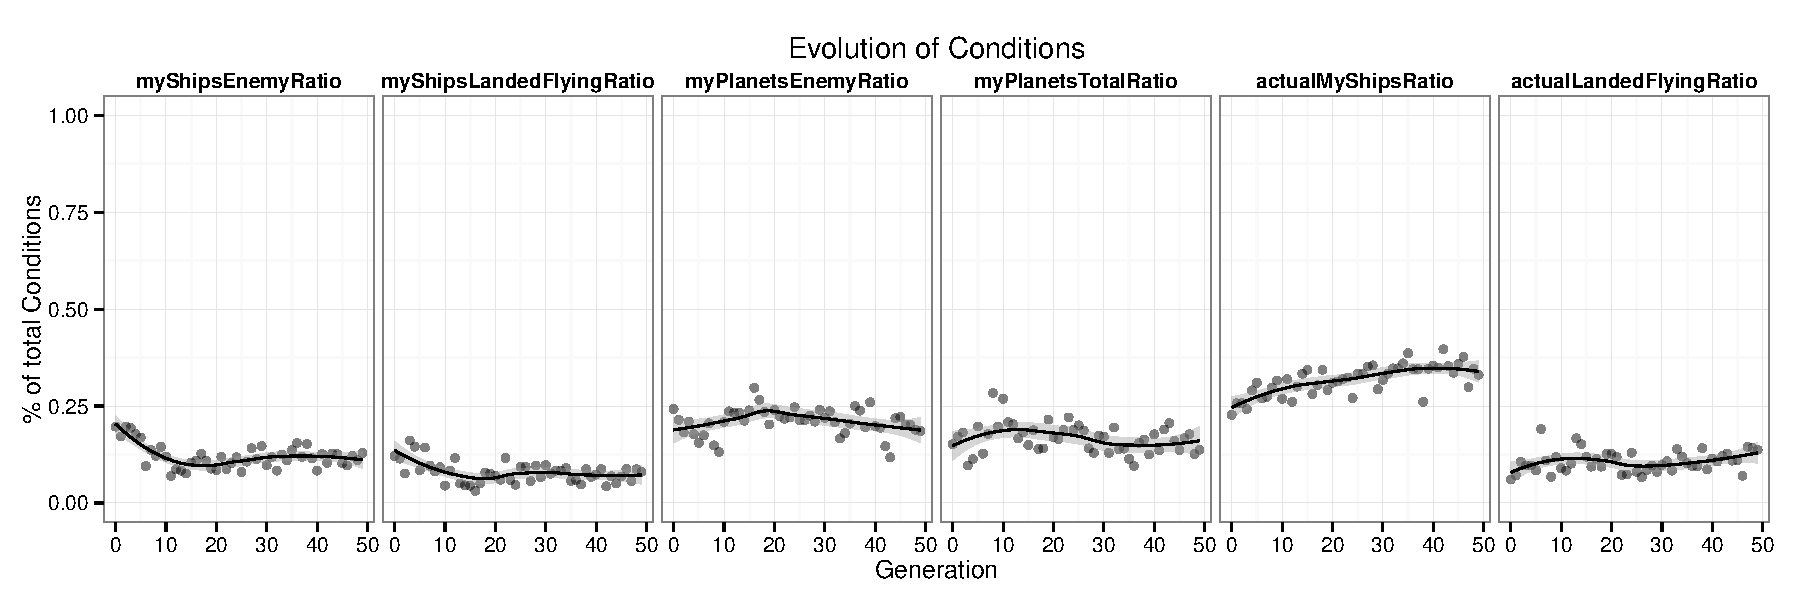
\includegraphics[width=12cm]{nuevas_imgs/estudio_CONDITIONS.pdf}
 \end{center}
 \caption{Evolution of the percentage of every conditions over the total of conditions used by the best individual by generation of every execution.}
 \label{figura:e_conditions}
 \end{figure}

 \begin{figure}[ht]
 \begin{center}
   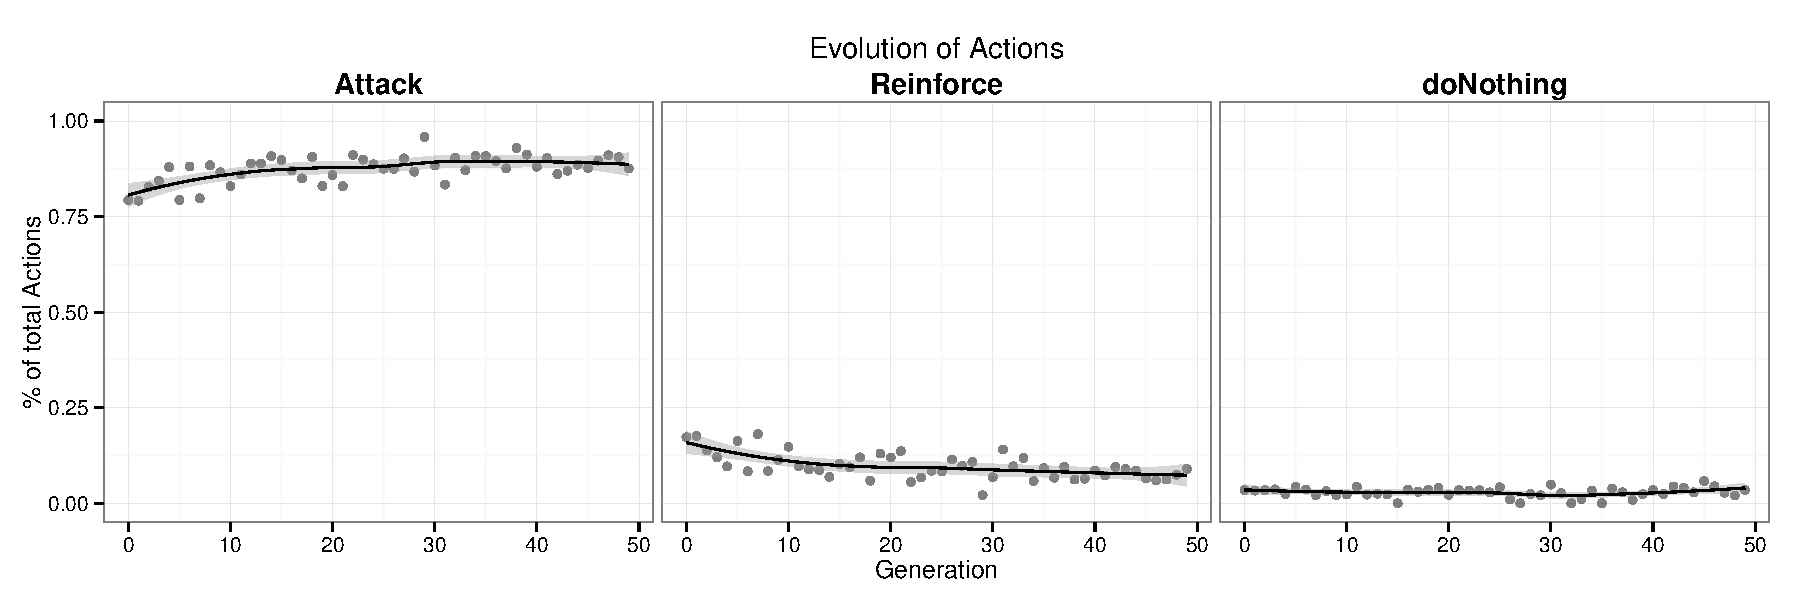
\includegraphics[width=12cm]{nuevas_imgs/estudio_ACTIONS.pdf}
 \end{center}
 \caption{Evolution of the percentage of every type of actions over the total of actions used by the best individual by generation of every execution. -- TO DO -- %Se puede ver que la acción más empleada por los mejores bots es la acción de atacar. Las acciones de reinforce y doNothing son menos usadas por los mejores bots a medida que se mejora la población.
 }
 \label{figura:e_actions}
 \end{figure}

 \begin{figure}[ht]
 \begin{center}
   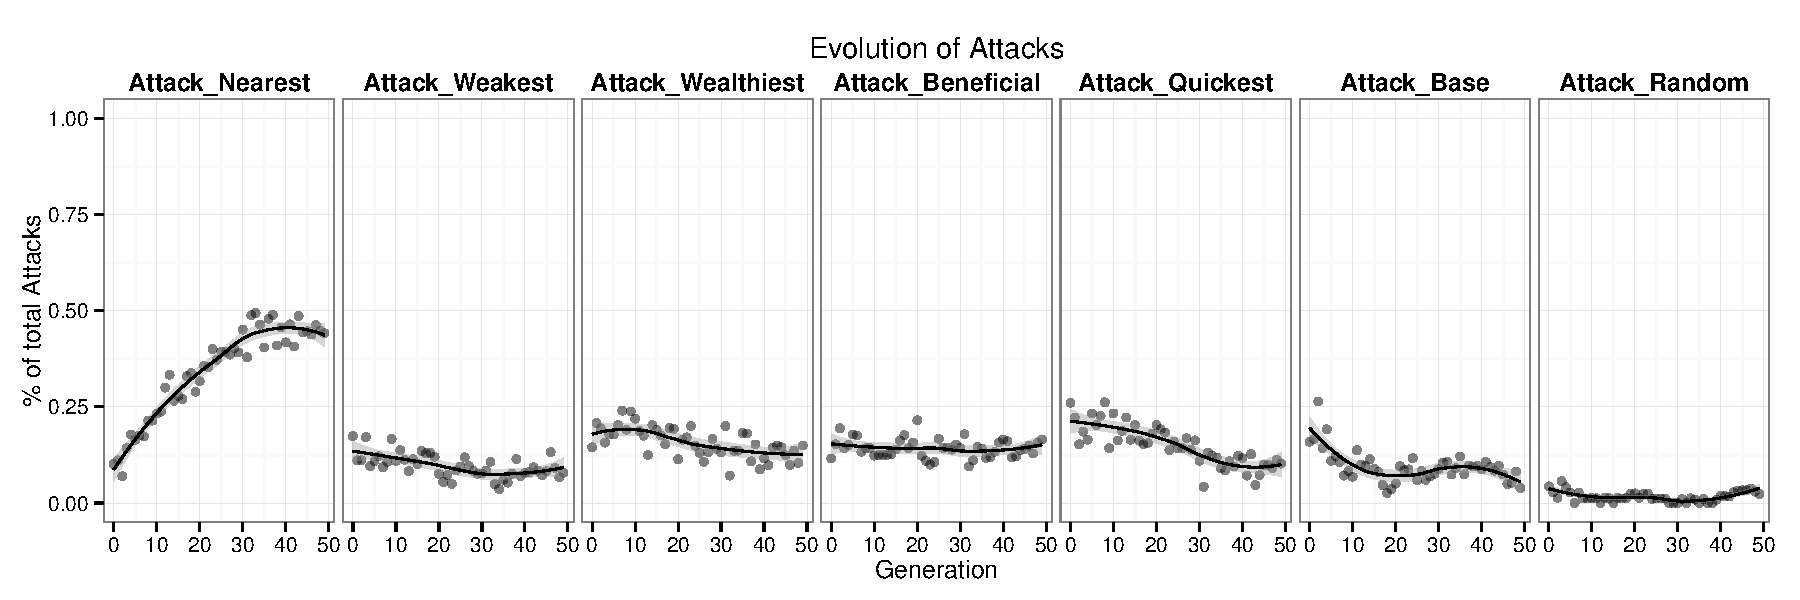
\includegraphics[width=12cm]{nuevas_imgs/estudio_ATTACKS.pdf}
 \end{center}
 \caption{Evolution of the percentage of every type of attack over the total of attacks used by the best individual by generation of every execution -- TO DO -- %Se puede observar como el attack de tipo attack_Nearest es el tipo de ataque más empleado por los mejores bots, por lo que se puede considerar que la mejores estretegia es atacar a los planetas más cercanos. Estrategias como attack_Base, attack_Quickest son menos usadas por los mejores bots a medida que mejora la población.
 }
 \label{figura:e_attacks}
 \end{figure}

  \begin{figure}[ht]
 \begin{center}
   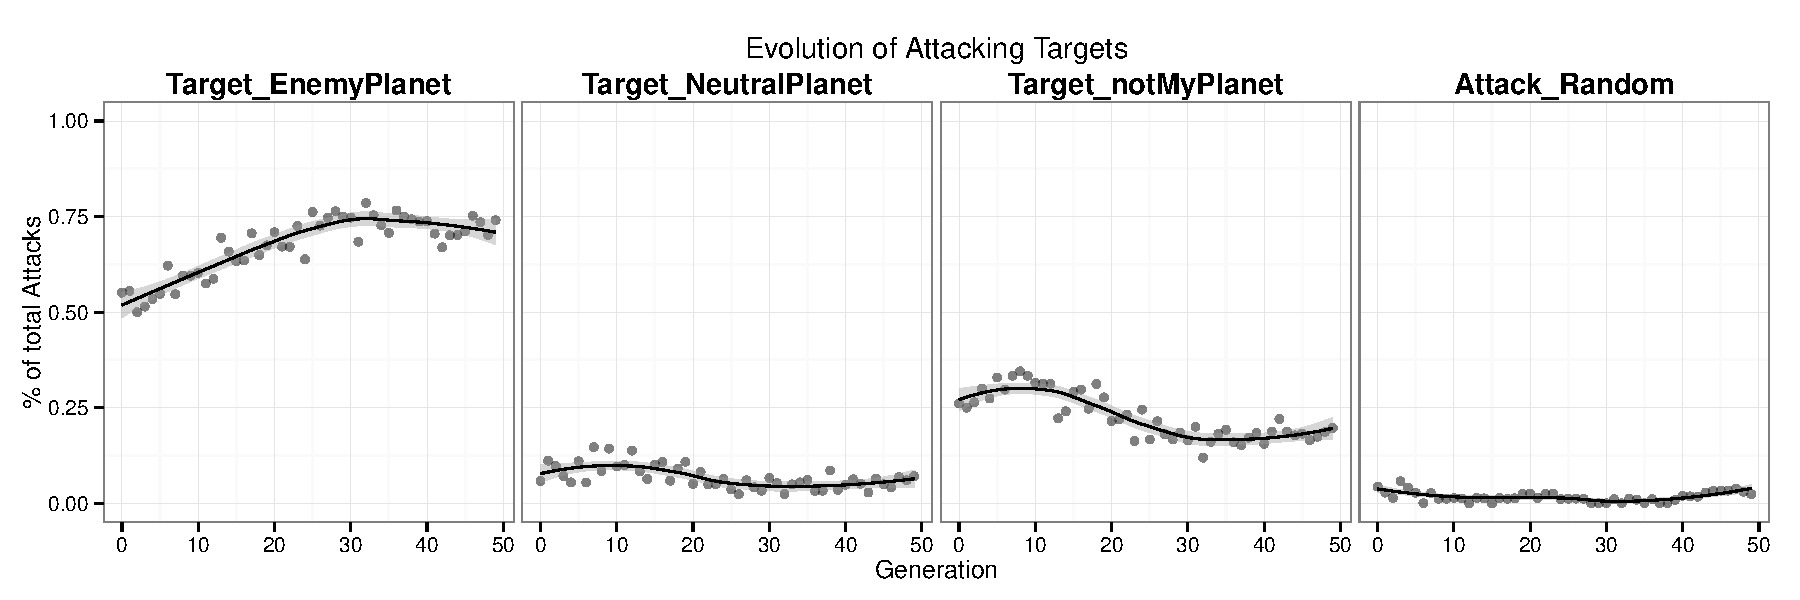
\includegraphics[width=12cm]{nuevas_imgs/estudio_TARGETS.pdf}
 \end{center}
 \caption{Evolution of the percentage of every type of attacking targets over the total of attaks used by the best individual by generation of every execution -- TO DO -- %Se puede ver como existen oscilaciones entre el atacar un planeta enemigo o un planeta neutral
 }
 \label{figura:e_targets}
 \end{figure}


   \begin{figure}[ht]
 \begin{center}
   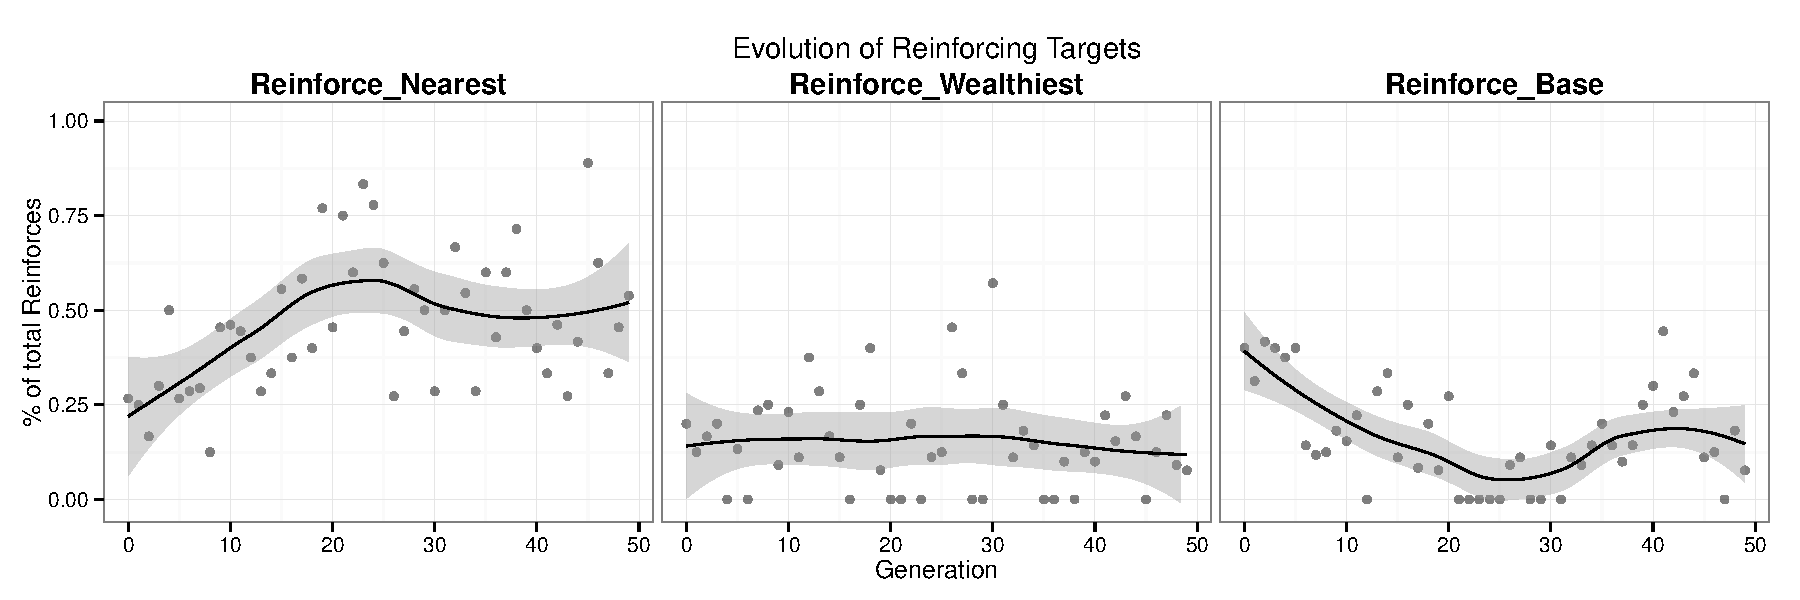
\includegraphics[width=12cm]{nuevas_imgs/estudio_TARGETS_REINFORCE.pdf}
 \end{center}
 \caption{Evolution of the percentage of every type of reinforce over
   the total of reinforces used by the best individual by generation
   of every execution -- TO DO--}
% What do you mean by reinforce? Refresh troops? - JJ 
 \label{figura:e_targetsReinforce}
 \end{figure}



%% DE AQUÍ PARA ABAJO ES TEXTO ANTIGUO DEL EVO QUE NO TIENE QUE VER CON ESTE ARTÍCULO

%FERGU: he borrado las tablas, que aquí no se usan. Dejo el resto comentado, por si queréis "inspiraros". Vamos, que no se reutiliza nada del trabajo del Evostar

%As can be seen, the average population fitness versus Genebot is nearest to the optimum than versus Exp-Genebot, even with the lowest depth. Highest performance in the population is also with the depth of 3 levels. On the contrary, confronting with Exp-Genebot the configuration with unlimited depth achieves better results. This make sense as more decisions should be taken because the enemy can be different in each map.

%In the second experiment, we have confronted the 30 bots obtained in each configuration again with Genebot and Exp-Genebot, but in the 100 maps provided by Google. This experiment has been used to validate if the obtained individuals of the proposed method can be competitive in terms of quality in maps not used for evaluation. Results are shown in Table \ref{tab:allmaps} and boxplots in Figure \ref{fig:victories}. %FERGU: si se va a hacer esto, esta frase se puede usar

%It can be seen that in average, the bots produced by the proposed algorithm perform equal or better than the best obtained by the previous authors. Note that, even obtaining individuals with maximum fitness (5 victories) that have been kept in the population several generations (as presented before in Tables \ref{tab:resultsGenebot} and \ref{tab:resultsExpgenebot}) cannot be representative of a extremely good bot in a wider set of maps that have not been used for training. As the distributions are not normalized, a Kruskal-Wallis test has been used, obtaining significant differences in turns for the experiment versus Genebot (p-value = 0.0028) and victories in Exp-genebot (p-value = 0.02681). Therefore, there are differences using a maximum depth in the generation of bots. In both configurations, the trees created with 7 levels of depth as maximum have obtained the better results.

%To explain why results versus Genebot (a weaker bot than Exp-Genebot) are slightly worse than versus Exp-Genebot, even when the best individuals produced by the GP have higher fitness, it is necessary to analyse how the best individual and the population are being evolved. Figure \ref{fig:gens} shows that best individual using Genebot reaches the optimal before Exp-Genebot, and also the average population converges quicker. This could lead to over-specialization: the generated bots are over-trained to win in the five maps. This is due because these individuals are being re-evaluated, and therefore, they are still changing after they have reached the optimal.



%\begin{table*}
%\centering{
%\begin{tabular}{|c|c|c|c|c|c|c|} \hline
   
%{\em Configuration}     &    {\em Average maps won}  &    {\em Average turns}     \\ \hline
%                   \multicolumn{3}{|c|}{Versus Genebot}    \\ \hline
% Depth 3          &   47.033 $\pm$ 10.001 &   133.371 $\pm$   16.34    \\ \hline
% Depth 7          &   48.9 $\pm$ 10.21    &   \textbf{141.386} $\pm$  15.54   \\ \hline
% Unlimited Depth  &   50.23 $\pm$ 11.40   &   133.916   $\pm$   10.55    \\ \hline
%       \multicolumn{3}{|c|}{Versus Exp-Genebot}                          \\ \hline              
% Depth 3          &   52.367 $\pm$ 13.39 &  191.051 $\pm$ 67.79 \\ \hline
% Depth 7          &   \textbf{58.867} $\pm$ 7.35  &  174.694$\pm$ 47.50 \\ \hline
% Unlimited Depth  &   52.3 $\pm$ 11.57   &  197.492 $\pm$ 72.30 \\ \hline 

%\end{tabular}


%\caption{Results confronting the 30 best bots attained from each configuration in the 100 maps each.}
%\label{tab:allmaps}
%}
%\end{table*}

%\begin{figure}[htb]
%\centering

%\subfigure[Victories]{
%   \includegraphics[scale =0.30] {imags/victories.eps}
%   \label{fig:subfig1}
% }
%\subfigure[Turns]{
%   \includegraphics[scale =0.30] {imags/turns.eps}
%   \label{fig:subfig2}
% }
%\caption{Average of executing the 30 best bots in each configuration (3, 7 and U) versus Genebot (G) and Exp-Genebot (E).}

%\label{fig:victories}
%\end{figure}

%\begin{figure}[htb]
%\centering
%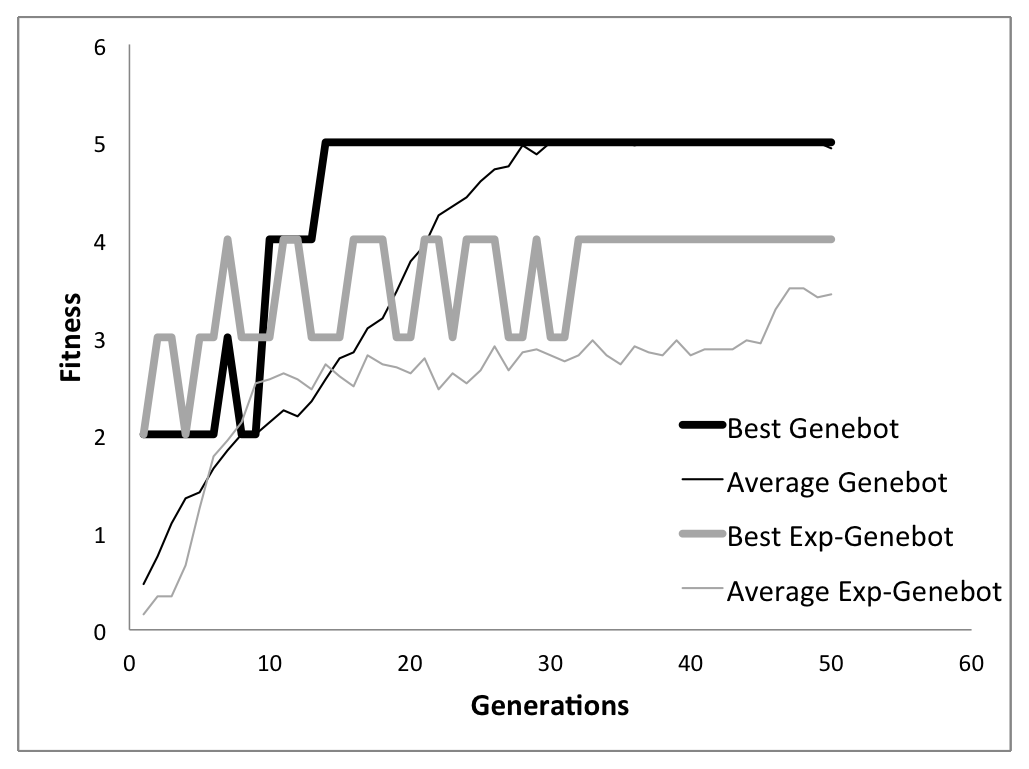
\includegraphics[scale =0.60] {imags/generations.eps}
%\caption{Evolution of the best individual and the average population during one run for depth 7 versus Genebot and Exp-Genebot.}
%\label{fig:gens}
%\end{figure}


%-----------------------------------------------------------------
%%%%%%%%%%%%%%%%%%%%%%%% CONCLUSIONS %%%%%%%%%%%%%%%%%%%%%%%%%%%%%
%----------------------------------------------------------------- 
\section{Conclusions}
\label{sec:conclusion}

%This work presents a Genetic Programming algorithm that generates agents for playing the Planet Wars game. A number of possible actions to perform and decision variables have been presented. A competitive bot available in the literature (Genebot) has been used to calculate the fitness of the generated individuals. This bot was the best obtained from several runs and the behaviour to be optimized was extracted from human expertise. %FERGU: confirmarlo %FERGU2: quitado exp-genebot y reescrito a continuación

%Genetic programming is a method that can help to create competitive bots for RTS games. % ?Eso es una conclusi?? ?Lo hab?s concluido en el paper? Empezad las conclusiones por "en este trabajo nos propon?mos probar..." - JJ
The objective of this work is to validate if using Genetic Programming
can create competitive bots for RTS games, %nobody has done it before?
                                %- JJ
 and study the behaviour of
% study behavior or find whichs fitness function is better? - JJ
different fitness functions, as they can affect directly to the
creation of these bots. Three different fitness functions have been
compared to generate bots for the Planet Wars game. A competitive bot
available in the literature (GeneBot) has been used to evaluate the
generated individuals (fighting against it). %Is this the best way of
                                %evaluating new bots? - JJ
 This bot was the best one
obtained in an evolutionary process which optimised different
parameters inside a human-designed behavioural engine.  


Different game metrics are taken into account in these functions to
obtain a metric to guide the evolution. %Although a turn-based fitness
                                %behaves more robustly than other
                                %methods, the area-based fitness
                                %achieves better percentage of
                                %victories in more produced robots. %
                                %robots o bots? - JJ 
%FERGU3: esto ultimo lo estoy escribiendo a las 3 de la mañana y no sé que pongo
% Por lo que más queráis, revisad el inglés - JJ FERGU4: ya, vaya horror.
The results show differences depending on the fitness used: % hey, big
                                % deal - JJ
 a victory-based fitness that prioritises the number of victories
 generates better bots on average than fitness that take into account
 the number of spaceships during all the run of the battle. % how
                                % many? 
This can
 be explained because this fitness exploits the individuals to
% exploits the individuals? really? - JJ
 generate more aggressive bots. However, their performance decreases
 confronting them versus different types of bots.  % so it is not so
                                % good? What gives? - JJ

% La conclusión tiene que estar relacionada con el título. ¿Qué habéis concluido con respecto a GP? ¿Qué tipo de GP? ¿Qué población? ¿No decís nada más que del fitness? - JJ FERGU

%Three different maximum depth for the trees have been used: 3, 7 and unlimited. Results show that the best individuals outperform these agents during the evolution in all configurations. These individuals have been tested against a larger set of maps not previously used during the evolution, obtaining equivalent or better results than Genebot and Exp-Genebot. FERGU: estos no son los resultados

%Results show that it is important to choose carefully the fitness that is going to be used to evaluate the evolved bots and to validate it using some kind of benchmark. % Some kind? Which kind? - JJ
% ¿Eso es lo único que muestran? - JJ FERGU4: joer, menuda mierda de frase he escrito...

As future lines of work, other rules will be added to the proposed algorithm
(for example, ones analysing the map) and more competitive enemies
will be used. In addition, the approach could be implemented and
tested in more complex RTS games, such as Starcraft, or even in
different videogames like Unreal\texttrademark~ or Super
Mario\texttrademark~. We will also use other ways of taking into
account the uncertainty in the fitness, such as using a Wilcoxon-based
method to compare them \cite{merelo2016statistical}. 

%%%%%%%%%%%%%%%%%%%%%%%%%%%%%  ACKNOWLEDGEMENTS %%%%%%%%%%%%%%%%%%%%%%%%%%%%%%%%
% TODO: actualizar con los nuevos proyectos
\section*{Acknowledgements}
% This work has been supported in part by projects 
% EPHEMECH (TIN2014-56494-C4-3-P, Spanish Ministerio de Econom? y Competitividad), 
% PROY-PP2015-06 (Plan Propio 2015 UGR), 
% PETRA (SPIP2014-01437, funded by Direcci? General de Tr?ico),
% CEI2015-MP-V17 (awarded by CEI BioTIC Granada), and 
% PRY142/14 (funded by Fundaci? P?blica Andaluza Centro de Estudios Andaluces en la IX Convocatoria de Proyectos de Investigaci?).

\bibliographystyle{elsarticle-num}
\bibliography{gpbot-fitness-entcom}
% is it so difficult to use the canonical geneura.bib file? 
% Why do you change the bib file??? - jj
\end{document}
